\documentclass[12pt,a4paper,notitlepage,twoside]{article}
\usepackage{polski}
\usepackage[utf8]{inputenc}
\usepackage{mathtools}
\usepackage{helvet}
\usepackage[top=2.5cm, bottom=2.5cm, left=3cm, right=2.5cm]{geometry}
\usepackage{caption}
\usepackage{subcaption}
\usepackage{graphicx}
\usepackage[absolute]{textpos}
\usepackage{tocloft}
\usepackage{cite}
\usepackage[numbib,notlof,notlot,nottoc]{tocbibind}
\usepackage{indentfirst}
\usepackage{fancyvrb}
\usepackage{listings}
\usepackage{float}
\linespread{1.3}
\usepackage[T1]{fontenc}
\usepackage{amssymb}
\renewcommand{\cftsecleader}{\cftdotfill{\cftdotsep}}
\renewcommand\figurename{Rys.}
%% \setlength\cftparskip{-2pt}
\setlength\cftbeforesecskip{1pt}
\setlength\cftaftertoctitleskip{2pt}

\lstset{
  numbers=left,
  breaklines=true,
  captionpos=b,
  language=C++,
  xleftmargin=\parindent,
  basicstyle=\small,
  inputencoding=utf8,
  escapeinside={\%*}{*)}
}

\usepackage{hyperref}
\hypersetup{
  colorlinks=true, %set true if you want colored links
  linktoc=all,     %set to all if you want both sections and subsections linked
  linkcolor=black,  %choose some color if you want links to stand out
  citecolor=black,
  urlcolor=black,
}

\setlength{\TPHorizModule}{10mm}
\setlength{\TPVertModule}{\TPHorizModule}
\textblockorigin{30mm}{25mm}

\makeatletter

\renewcommand{\maketitle}{\begin{titlepage}

    \begin{center}
      
\includegraphics[width=2.5cm]{img/polsl-logo}
    \end{center}

    \vspace{0.5cm}
    \begin{center}
      \Large{\textbf{\textsc{Politechnika Śląska\\
	    Wydział Automatyki, Elektroniki i Informatyki\\
	    Kierunek Informatyka\\}}}
    \end{center}

    \vspace{1.35cm}
    \begin{center}
      \Large{Praca dyplomowa magisterska}
    \end{center}

    \begin{center}

      \vspace{1.5cm}
      {\fontsize{14}{36}\selectfont \@title}

    \end{center}

    \begin{textblock}{10}(0,19)
      \noindent{\fontsize{14}{21}{Autor: \@author\\
	  Kierujący pracą: prof. dr hab. inż. Stanisław Kozielski\\
	  Konsultant: dr inż. Zbigniew Szaszkowski}}
    \end{textblock}
    \begin{textblock}{15.5}(0,24)
      \begin{center}
	Gliwice, czerwiec 2015
      \end{center}
    \end{textblock}
  \end{titlepage}

}

\makeatother

\author{Marcin Kolny}

\title{Rozpoznawanie ciągów znaków z wykorzystaniem metod segmentacji obrazu}
\renewcommand{\familydefault}{\sfdefault}
\begin{document}
\maketitle
\newpage
\tableofcontents
\newpage
\section{Wstęp}
Analiza obrazu odgrywa coraz większą rolę w~szeroko pojętej inspekcji obiektów. Dzięki algorytmom wizji komputerowej systemy informatyczne są coraz częściej wykorzystywane w~przemyśle, w~miejscach gdzie do tej pory pracę musiał wykonywać człowiek. Systemy oparte o~analizę wizji komputerowej mogą pracować o~wiele wydajniej oraz popełniają o~wiele mniej błędów. Ponadto są tanie w~utrzymaniu. Standardem jest już na przykład inspekcja wizyjna jakości na taśmach produkcyjnych. Przykładem wykorzystania wizji komputerowej w~rozwiązaniach przemysłowych może być weryfikacja butelki oddanej do automatu przyjmującego butelki zwrotne. System na podstawie zdjęcia może stwierdzić, czy kształt butelki jest akceptowany w~danej maszynie oraz czy butelka nie jest uszkodzona, i~w zależności od rezultatu oceny, wypłacić użytkowi pieniądze lub zwrócić butelkę.
\paragraph{}
Segmentacja odgrywa ważną rolę w~analizie obrazu, ponieważ pozwala na wyodrębnienie z~obrazu cech, które są istotne z~punktu widzenia danego problemu. Na obrazie, na którym zarejestrowany jest badany obiekt, znajdują się bardzo często inne obiekty, które są zbędne z~punktu widzenia rozwiązania danego problemu, a~nawet przeszkadzają w~jego rozwiązaniu. Zadaniem segmentacji jest wydobycie z~obrazu tylko takich obiektów, które mogą być przydatne w~kolejnym etapie, jakim jest analiza obiektu.
\paragraph{}
Metody segmentacji są jednym ze sposobów rozpoznawania ciągów znaków. Dzięki metodom segmentacji możemy z~pośród całego tekstu wyodrębnić zbiór pojedynczych znaków, a~następnie przekazać je do algorytmu rozpoznawania pojedynczych znaków.
\paragraph{}
Celem mojej pracy jest zaprezentowanie podstawowych algorytmów przetwarzania wizji komputerowej oraz metod segmentacji obrazów. Metody segmentacji omówię pod kątem rozwiązywania problemu segmentacji tekstu, a~w szczególnym przypadku - segmentacji obrazów tablic rejestracyjnych pojazdów. Przedstawię problemy, jakie wiążą się z~zagadnieniem segmentacji obrazów tablic rejestracyjnych, oraz omówię zaproponowane przeze mnie rozwiązania tych problemów. Głównym celem jest porównanie pod względem jakościowym algorytmów segmentacji obrazu w~zastosowaniu segmentacji obrazów tablic rejestracyjnych pojazdów. Dlatego omówię algorytmy, jakie zdecydowałem się wykorzystać do przeprowadzenia badań. Następnie przedstawię sposób, w~jaki przeprowadzałem badania, omówię środowisko, jakie przygotowałem w~celu przeprowadzenia testów algorytmów. Na końcu mojej pracy zaprezentuję uzyskane przeze mnie wyniki.
\paragraph{}
Na początku pracy opisałem podstawowe operacje wykonywane na obrazach, wprowadziłem pojęcia, których będę używał w~dalszych rozdziałach. Następnie przedstawiłem problem segmentacji obrazu oraz zaprezentowałem metody służące do segmentacji obrazu. W~dalszej części pracy przedstawiłem algorytmy rozpoznawania znaków. Następnie wymieniłem problemy związane z~segmentacją obrazów tablic rejestracyjnych, a~także zaproponowałem metody rozwiązywania tych problemów. W~kolejnym rozdziale przedstawiłem proces badania metod segmentacji obrazów tablic rejestracyjnych, opisałem algorytmy poddane badaniom. Na końcu pracy zaprezentowałem i~porównałem wyniki moich badań, a~także podsumowałem moją pracę.

\newpage
\section{Analiza obrazu}
\subsection{Podstawowe informacje dotyczące przetwarzania obrazów}
\subsubsection{Tryb koloru}
Określenie sposobu reprezentacji kolorów w obrazach rastrowych nazywamy \textbf{trybem koloru}. Wyróżniamy następujące tryby koloru:
\begin{itemize}
  \item czarno-biały - w obrazie występują tylko kolory: biały i czarny,
  \item skala szarości - oprócz koloru czarnego i białego, występuje cała gama jasności pośrednich,
  \item tryb kolorowy - piksele mają przyporządkowane kolory z przestrzeni barw.
\end{itemize}
Symbolem $I$ będziemy oznaczać zbiór kolorów. Dla trybu czarno-białego
\begin{gather*}
  I = \{0, 1\}
\end{gather*} gdzie 0 reprezentuje kolor czarny, a 1 kolor biały.\\
Dla trybu skali szarości
\begin{gather*}
  I = \{0, 1, ..., 2^b-1\}
\end{gather*}
gdzie $b$ jest liczbą bitów potrzebnych do reprezentacji jasności, 0 oznacza kolor czarny, $2^b-1$ kolor biały, a pozostałe wartości opisują jasność koloru. Najczęściej wartość $b$ jest wielokrotnością liczby 8.\\
Dla trybu kolorowego
\begin{gather*}
  I = I_1 \times I_2 \times ... \times I_n,
\end{gather*}
gdzie
\begin{gather*}
  I_1 = I_2 = ... = I_n = \{0, 1, ..., 2^b-1\}
\end{gather*}
oraz $n\in \mathbb{N} \wedge n > 1$ jest liczbą kanałów z przestrzeni barw. \\
Dla przestrzeni barw RGB
\begin{gather*}
  I = I_R \times I_G \times I_B
\end{gather*}
gdzie $I_R$, $I_G$, $I_B$ oznaczają odpowiednio jasność kolorów czerwonego, zielonego i niebieskiego. Przestrzeń RGB jest trzykanałowa.
\subsubsection{Obraz cyfrowy}
Obraz cyfrowy definiujemy jako funkcję
\begin{gather*}
  f: \{0, 1, ..., N-1\} \times \{0, 1, ..., M-1\} \rightarrow I,
\end{gather*}
gdzie $M$, $N$ oznaczają odpowiednio szerokość i wysokość obrazu.\\
Wartość funkcji $f(x, y)$ nazywamy \textbf{pikselem}.\\
Obrazy cyfrowe możemy podzielić ze względu na tryb opisu koloru:
\begin{itemize}
  \item czarno-białe,
  \item jednokanałowe (monochromatyczne),
  \item wielokanałowe (kolorowe).
\end{itemize}
Na rysunku~\ref{fig:image_examples} przedstawione zostały obrazy w których zastosowano wyżej wymienione tryby opisu koloru.\\
Symbolem $P_{N,M}$ będziemy oznaczać zbiór
\begin{gather*}
  P_{N,M} = \{0, 1, ..., N-1\} \times \{0, 1, ..., M-1\}.
\end{gather*}
Każdy obraz cyfrowy $P = (P_{N,M}; f; I)$ opisuje trójka\\
$P_{N,M}$ - zbiór współrzędnych punktów obrazu,\\
$I$ - zbiór opisujący kolor obrazu,\\
$f$ - funkcja przyporządkowująca punktowi kolor.

\begin{figure}
  \centering
  \begin{subfigure}[b]{0.45\textwidth}
    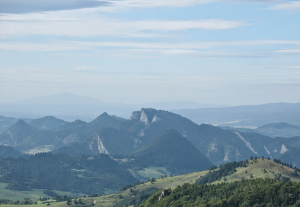
\includegraphics[width=\textwidth]{img/basics-image-color}
    \caption{Trzykanałowy obraz cyfrowy (kolorowy)}
    \label{fig:basics_image_color}
  \end{subfigure}
  ~
  \begin{subfigure}[b]{0.45\textwidth}
    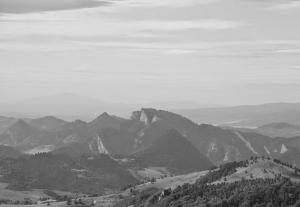
\includegraphics[width=\textwidth]{img/basics-image-gray}
    \caption{Jednokanałowy obraz cyfrowy (monochromatyczny)}
    \label{fig:basics_image_gray}
  \end{subfigure}
  ~
  \begin{subfigure}[b]{0.45\textwidth}
    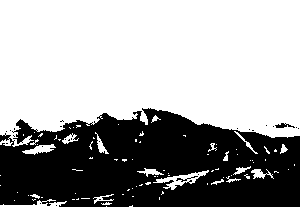
\includegraphics[width=\textwidth]{img/basics-image-binary}
    \caption{Obraz jednokanałowy (czarno-biały)}
    \label{fig:basics_image_binary}
  \end{subfigure}
  \caption{Obrazy cyfrowe wykorzystujące różne tryby kolorów}\label{fig:image_examples}
\end{figure}
\subsection{Podstawowe operacje przetwarzania obrazów}
Symbolem
\begin{gather*}
  P^{(in)} = (P_{N,M}^{(in)}, f^{(in)}, I^{(in)})
\end{gather*}
oznaczamy obraz wejściowy, a 
\begin{gather*}
  P^{(out)} = (P_{N,M}^{(out)}, f^{(out)}, I^{(out)})
\end{gather*}
obraz wyjściowy.

\subsubsection{Kadrowanie obrazu}
Operacja kadrowania polega na pozostawieniu na obrazie wejściowym tylko tych pikseli, które znajdują się w zdefiniowanym prostokątnym obszarze. Obraz wyjściowy po operacji kadrowania przyjmuje rozmiar obszaru, do którego kadrowany był obraz wejściowy.\\
Na rysunku~\ref{fig:crop_image} przedstawiona została operacja kadrowania obrazu. Celem kadrowania jest usunięcie z obrazu informacji, które są zbędne podczas wykonywania analizy obrazu, ponieważ mogą negatywnie wpłynąć na czas oraz rezultaty wykonania algorytmów.
\begin{figure}
  \centering
  \begin{subfigure}[b]{0.45\textwidth}
    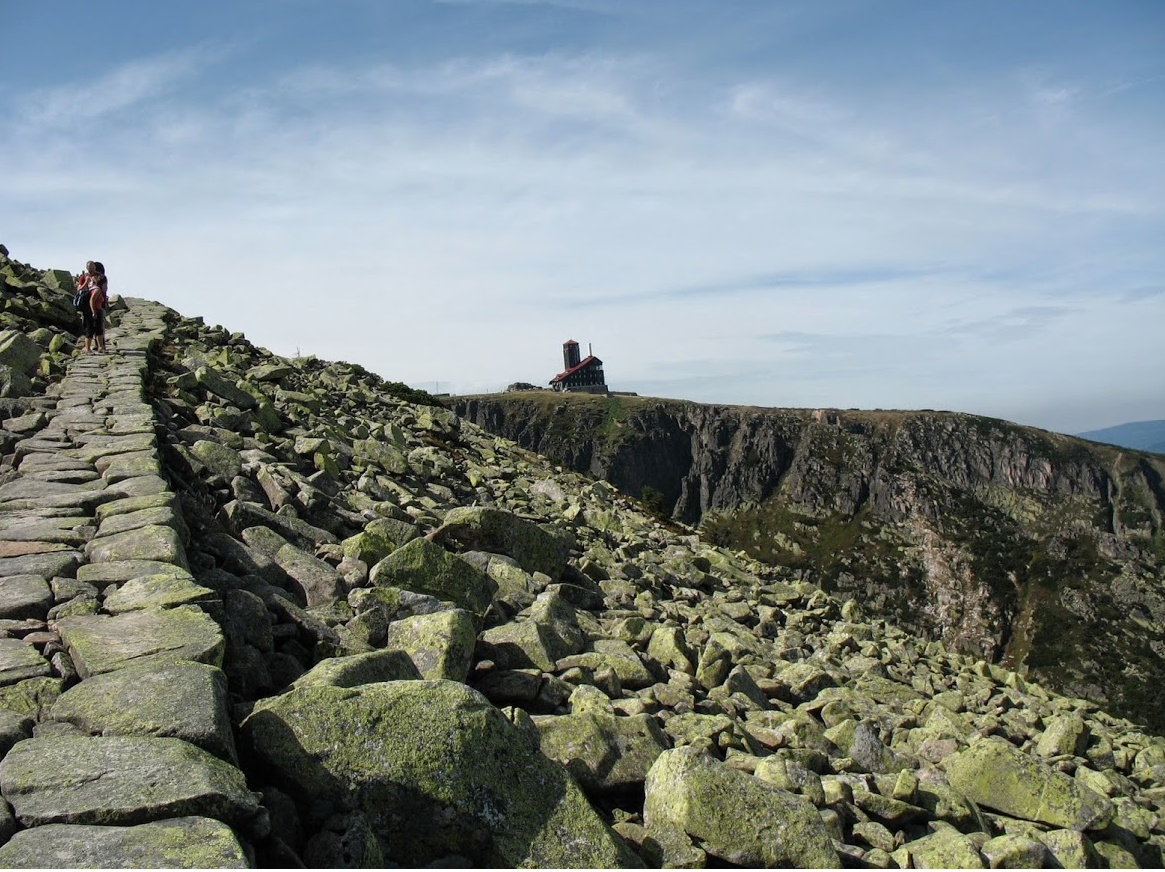
\includegraphics[width=\textwidth]{img/crop-image-before}
    \caption{Obraz wejściowy dla operacji kadrowania}
    \label{fig:crop_image_before}
  \end{subfigure}
  ~
  \begin{subfigure}[b]{0.45\textwidth}
    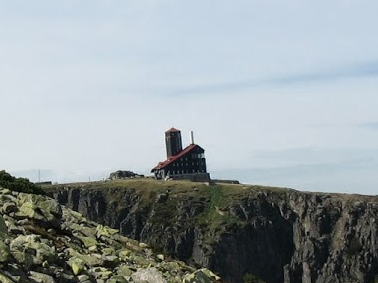
\includegraphics[width=\textwidth]{img/crop-image-after}
    \caption{Obraz wyjściowy, poddany operacji kadrowania}
    \label{fig:crop_image_after}
  \end{subfigure}
  \caption{Operacja kadrowania obrazu}\label{fig:crop_image}
\end{figure}
\subsubsection{Progowanie (binaryzacja)} \label{sssec:threshold}
Progowanie polega na podziale pikseli obrazu na dwie grupy, poprzez wybranie określonej wartości progowej $t$. Każdy piksel jest porównywany z wartością progową, i w zależności od tego, czy wartość piksela jest większa od wartości progowej, czy mniejsza, w tej samej pozycji nowo powstałego obrazu, przypisuje się wartość $1$, lub $0$. Operację można opisać wzorem:
\begin{gather*}
  f^{(out)}(x, y) = \left\{\begin{matrix}
  1, dla \: f^{(in)}(x, y) > t,\\
  0, dla \: f^{(in)}(x, y) \leq t,
  \end{matrix}\right. \quad (x, y) \in P^{(in)}_{N,M}
\end{gather*}
Na rysunku~\ref{fig:threshold_image} przedstawiony został wynik operacji progowania na przykładowym obrazie monochromatycznym.
\begin{figure}
  \centering
  \begin{subfigure}[b]{0.45\textwidth}
    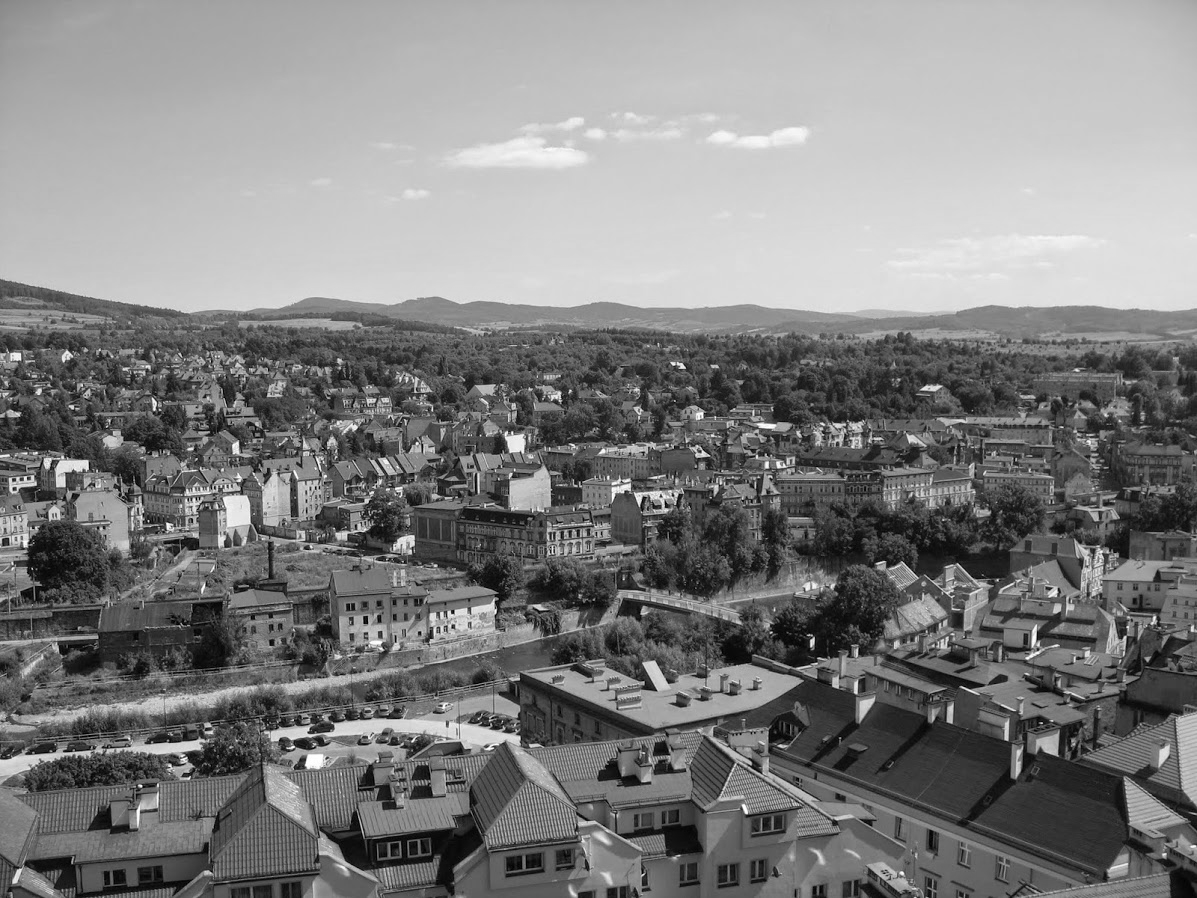
\includegraphics[width=\textwidth]{img/threshold-before}
    \caption{Obraz wejściowy dla operacji progowania}
    \label{fig:threshold_before}
  \end{subfigure}
  ~
  \begin{subfigure}[b]{0.45\textwidth}
    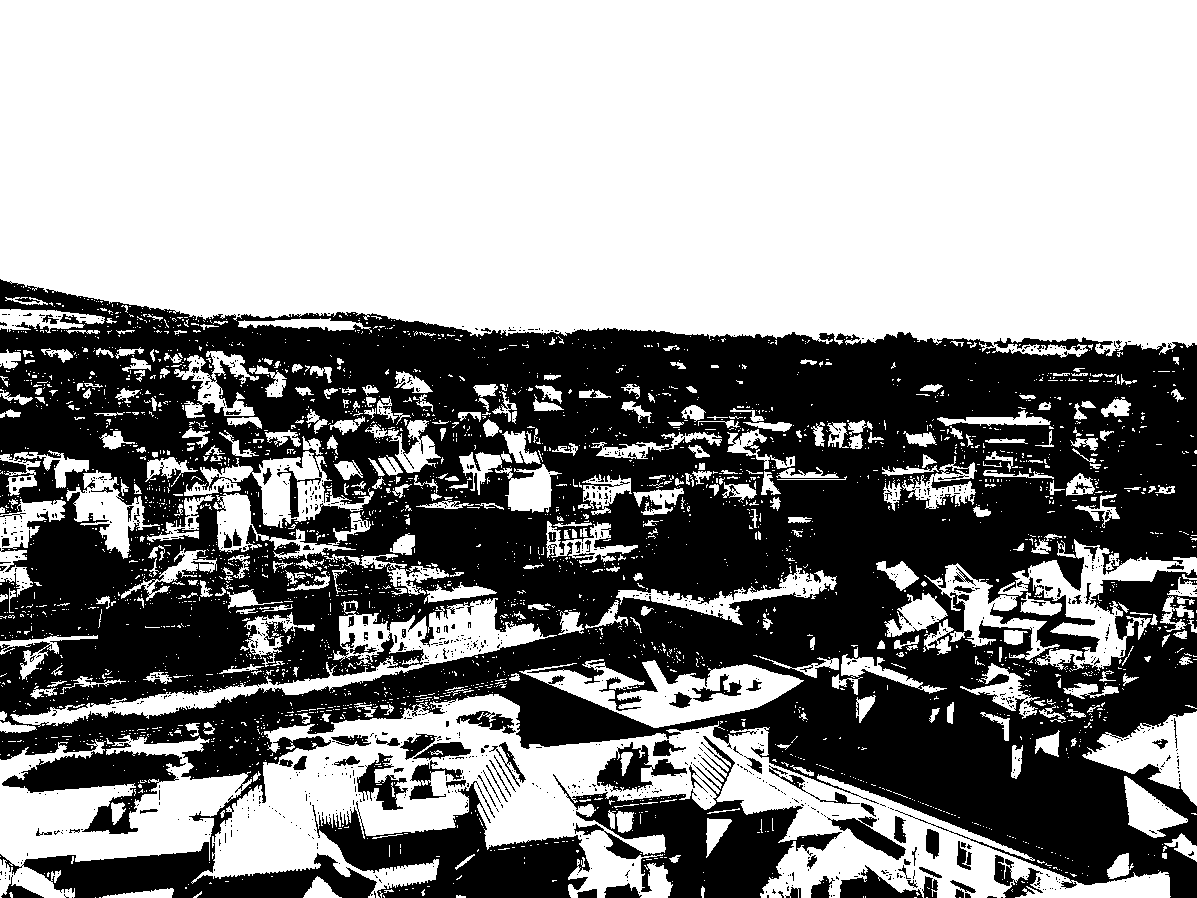
\includegraphics[width=\textwidth]{img/threshold-after}
    \caption{Obraz wyjściowy, poddany operacji progowania}
    \label{fig:threshold_after}
  \end{subfigure}
  \caption{Operacja progowania z wartością progu $t=128$ dla obrazu jednokanałowego}\label{fig:threshold_image}
\end{figure}

\paragraph{Progowanie obrazów wielokanałowych}\mbox{}\\
Zazwyczaj operacji progowania poddawane są obrazy jednokanałowe. Istnieje jednak możliwość wykonania operacji progowania dla obrazów wielokanałowych (np. dla obrazów RGB). Operacja ta definiowana jest następującym wzorem:
\begin{gather*}
  f^{(out)}(x, y) = \left\{\begin{matrix}
  1, \; \text{jeżeli} \; \forall c \in C, \; f^{(in)}(x, y, c) > t(c),\\
  0, \; \text{jeżeli} \; \exists c \in C, \; f^{(in)}(x, y, c) \leq t(c),
  \end{matrix}\right. \quad (x, y) \in P^{(in)}_{N,M} c=0,1,2,...,C,
\end{gather*}
gdzie $C$ to liczba kanałów w obrazie.
Algorytm progowania operujący na wielu kanałach może zostać wykorzystany, kiedy znana jest dokładna barwa badanego obiektu.

\paragraph{Progowanie lokalne}\mbox{}\\
Progowanie lokalne znajduje zastosowanie w przypadku gdy obraz jest niejednolicie oświetlony. Trudno jest dobrać globalny próg w taki sposób, aby wyekstrachować z obrazu nawet większość porządanych obiektów. Progowanie lokalne polega na wyznaczeniu danego progu w sąsiedztwie aktualnie przetwarzanego piksela. 
\begin{gather*}
  f^{(out)}(x, y) = \left\{\begin{matrix}
  1, dla \: f^{(in)}(x, y) > T(x, y),\\
  0, dla \: f^{(in)}(x, y) \leq T(x, y),
  \end{matrix}\right. \quad (x, y) \in P^{(in)}_{N,M},
\end{gather*}
gdzie $T(x, y)$ to funkcja zwracająca próg w zadanym sąsiedztwie piksela o współrzędnych $(x, y)$. Zwykle jako funkcję wyznaczania progu przyjmuje się wartość średnią lub sumą ważoną, wykorzystującą krzywą Gaussa.

\subsubsection{Filtracja obrazu}
Poprzez \textbf{jądro (maskę)} w kontekscie przetwarzania obrazów rozumiemy kształt którym parametryzowana jest operacja filtracji obrazu. Symbolami $k_N$, $k_M$ będę oznaczał rozmiar jądra (kolejno wysokość oraz szerokość).\\
Operacje filtracji mają na celu wykonanie zadanego przekształcenia matematycznego dla każdego piksela, generując tym samym nowy obraz. Filtrację obrazu stosuje się zwykle w celu wydobycia z obrazu żądanych informacji lub usunięcia szumu. Poniżej wymienionych zostało kilka najczęściej używanych operacji filtrowania obrazu:
\begin{itemize}
\item filtr uśredniający - stosowany jest w celu rozmycia obrazu
  \begin{gather*}
    f^{(out)}(x, y) = \frac{\sum\limits_{x=M-k_\frac{M}{2}}^{M+\frac{k_M}{2}} \sum\limits_{y=N-\frac{k_N}{2}}^{N+\frac{k_N}{2}} f^{(in)}(x, y)}{k_M \cdot k_N}, \quad (x, y) \in P^{(in)}_{N,M},
  \end{gather*}
\item filtr medianowy - wykorzystywany jest do usuwania zakłóceń na obrazie
  \begin{gather*}
    f^{(out)}(x, y) = mediana(\{f^{(in)}(x, y), \;x \in \big< M-\frac{k_x}{2}, M+\frac{k_x}{2}\big> \\
    \wedge\; y \in \big< N-\frac{k_y}{2}, N+\frac{k_y,}{2}\big>\}), \quad (x, y) \in P^{(in)}_{N,M},
  \end{gather*}
\item filtr Gaussa - podobnie jak filtr uśredniający, filtr Gaussa stosuje się do redukcji detali na obrazie poprzez jego rozmycie
  \begin{gather*}
    f^{(out)}(x, y) = \frac{1}{\sqrt{2 \pi \sigma}} e^{-\frac{x^2+y^2}{2 \sigma^2}}, \quad (x, y) \in P^{(in)}_{N,M}.
  \end{gather*}
\end{itemize}

Rysunek~\ref{fig:lena_smooth} przedstawia zaszumiony obraz oraz wynik działania algorytmu rozmycia medianowego.
\begin{figure}
  \centering
  \begin{subfigure}[b]{0.45\textwidth}
    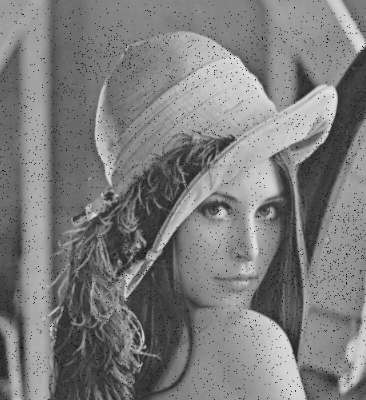
\includegraphics[width=\textwidth]{img/smooth-lena-input}
    \caption{Obraz wejściowy}
    \label{fig:smooth_lena_input}
  \end{subfigure}
  ~
  \begin{subfigure}[b]{0.45\textwidth}
    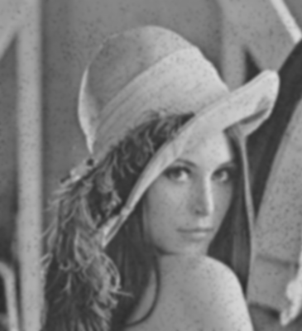
\includegraphics[width=\textwidth]{img/smooth-lena-gauss}
    \caption{Operacja rozmycia Gaussa}
    \label{fig:smooth_lena_gauss}
  \end{subfigure}
  ~
  \begin{subfigure}[b]{0.45\textwidth}
    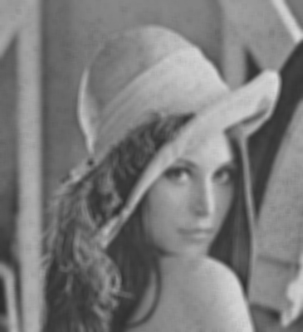
\includegraphics[width=\textwidth]{img/smooth-lena-mean}
    \caption{Operacja rozmycia średniego}
    \label{fig:smooth_lena_gauss}
  \end{subfigure}
  ~
  \begin{subfigure}[b]{0.45\textwidth}
    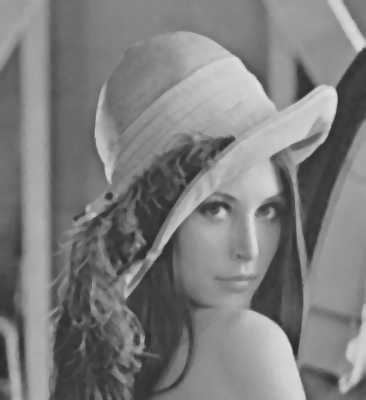
\includegraphics[width=\textwidth]{img/smooth-lena-median}
    \caption{Operacja rozmycia medianowego}
    \label{fig:smooth_lena_gauss}
  \end{subfigure}
  \caption{Wynik działania podstawowych operacji rozmycia na obrazie wejściowym}
  \label{fig:lena_smooth}
\end{figure}
\subsubsection{Dodawanie obrazów}
W tym podrozdziale, jako $n$ oznaczać będziemy liczbę obrazów wejściowych poddawanych operacji dodawania, jako $P^{(in)}_{i}$ będziemy rozumieć $i-ty$ obraz wejściowy, natomiast poprzez $f^{(in)}_i$ będziemy oznaczać funkcję $i-tego$ obrazu przyporządkowującą punktowi kolor. Symbolem $w_i$ będziemy oznaczać wagę przyporządkowaną do $i-tego$ obrazu wejściowego.\\
Operacja dodawania obrazów 
\begin{gather*}
P^{(out)} = P_1^{(in)} + P_2^{(in)} + ... + P_n^{(in)}
\end{gather*}
definiowana jest wzorem:
\begin{gather*}
  f^{(out)}(x, y) = \displaystyle\sum_{i=1}^{n} f^{(i)}(x, y), \quad (x, y) \in P^{(in)}_{N,M}.
\end{gather*}
\paragraph{Dodawanie obrazów z wagami} \mbox{}\\
Dodawanie obrazów z wagami zdefiniowane jest wzorem:
\begin{gather*}
  f^{(out)}(x, y) = \displaystyle\sum_{i=1}^{n} f^{(in)}_i(x, y) \cdot w_i, \quad (x, y) \in P^{(in)}_{N,M}.
\end{gather*}
\subsubsection{Wyostrzenie obrazu}
W celu uzyskania efektu wyostrzonych krawędzi obrazu, należy wykonać na obrazie wejściowym operację rozmycia Gaussa, a następnie obraz wynikowy dodać do obrazu wejściowego z wagami:
\begin{itemize}
  \item 1.5 dla obrazu wejściowego,
  \item -0.5 dla obrazu poddanego operacji rozmycia Gaussa.
\end{itemize}Na rysunku~\ref{fig:image_sharpen} przedstawiono obraz poddany operacji wyostrzania, oraz wynik tej operacji.
\begin{figure}
  \centering
  \begin{subfigure}[b]{0.45\textwidth}
    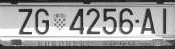
\includegraphics[width=\textwidth]{img/image-sharpen-before}
    \label{fig:image_sharpen_before}
  \end{subfigure}
  ~
  \begin{subfigure}[b]{0.45\textwidth}
    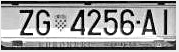
\includegraphics[width=\textwidth]{img/image-sharpen-after}
    \label{fig:image_sharpen_after}
  \end{subfigure}
  \caption{Operacja wyostrzenia wykonana na obrazie jednokanałowym}
  \label{fig:image_sharpen}
\end{figure}
\subsubsection{Normalizacja obrazu}
W tym podrozdziale jako $\min_{in}$ oraz $max_{in}$ będziemy oznaczać minimalną i maksymalną wartość funkcji jasności obrazu wejściowego, natomiast jako $\min_{out}$ oraz $min_{out}$ będziemy oznaczać minimalną i maksymalną pożądaną wartość funkcji jasności obrazu wyjściowego. \\
Operacja normalizacji służy do zmiany przedziału wartości pikseli występujących w obrazie, i definiowana jest wzorem:
\begin{gather*}
  f^{(out)}(x, y) = (f^{(in)}(x, y) - min_{in}) \cdot \frac{max_{out} - min_{out}}{max_{in} - min_{in}}+min_{in}, \quad \quad (x, y) \in P^{(in)}_{N,M}.
\end{gather*}
Rysunek~\ref{fig:image_normalize} prezentuje działanie algorytmu normalizacji. Obraz wejściowy został wykonany w bardzo ciemnym otoczeniu, natomiast po wykonaniu operacji kontrast obrazu został poprawiony.
\begin{figure}
  \centering
  \begin{subfigure}[b]{0.45\textwidth}
    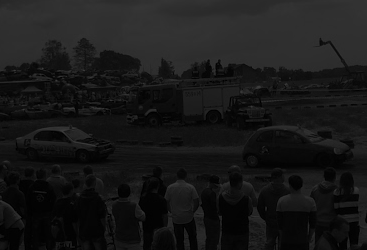
\includegraphics[width=\textwidth]{img/image-normalize-before}
    \label{fig:image_normalize_before}
  \end{subfigure}
  ~
  \begin{subfigure}[b]{0.45\textwidth}
    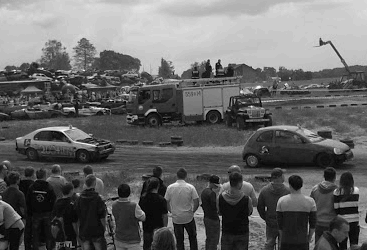
\includegraphics[width=\textwidth]{img/image-normalize-after}
    \label{fig:image_normalize_after}
  \end{subfigure}
  \caption{Normalizacja obrazu}
  \label{fig:image_normalize}
\end{figure}
\subsection{Operacje morfologiczne}
Operacje morfologiczne na obrazach wykorzystywane są do filtracji morfologicznej oraz analizy kształtów obiektów na obrazie. Definiują one zbiór punktów, jakie powinny pozostać na obrazie. W praktyce jest to realizowane poprzez ustawianie wartości jasności danego piksela na wartość 0 w przypadku nieistnienia danego punktu w zbiorze, lub wartości maksymalnej dla funkcji jasności, jeśli piksel o danych współrzędnych znajduje się w zbiorze. Przekształcenia morfologiczne są podstawą dla wielu bardziej złożonych algorytmów wizji komputerowej.\\
Jako symbol $A$ będziemy oznaczali zbiór punktów w których obraz wejściowy posiada wartość jasności równą 1, symbol $B$ będzie reprezentował maskę dla operacji morfologicznej. Funkcja $translacja(a, b)$ definiuje przesunięcie elementu strukturalnego (maski) $a$ na pozycję określoną przez współrzędne $b$.
\subsubsection{Dylatacja obrazu}
Dylatacja to rozszerzenie obrazu wykorzystując zadaną maskę. Operacja definiowana jest wzorem
\begin{gather*}
  A \oplus B \equiv \{ (x, y) \in A | A \cap translacja(B, (x, y)) \neq \emptyset \}.
\end{gather*}
Przykładowy wynik operacji dylatacji przedstawiony jest na rysunku~\ref{fig:dilate}.
\begin{figure}
  \centering
  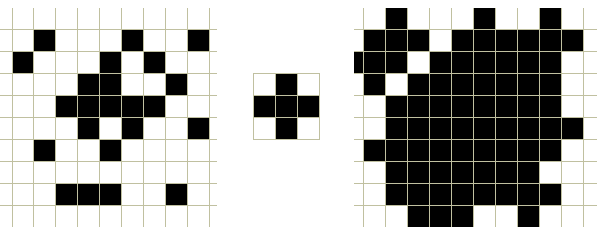
\includegraphics[width=15cm]{img/dilate}
  \caption{Obraz binarny poddany procesowi dylatacji z zadanym elementem strukturalnym}
  \label{fig:dilate}
\end{figure}
\subsubsection{Erozja obrazu} 
Erozja obrazu polega na zwężaniu obrazu z wykorzystaniem zadanego elementu strukturalnego. Operacja definiowana jest wzorem
\begin{gather*}
  A \ominus B \equiv \{ (x, y) \in A | translacja(B, (x, y) \subset A \}.
\end{gather*}
Przykładowy wynik operacji erozji obrazu przedstawiony został na rysunku~\ref{fig:erode}.
\begin{figure}
  \centering
  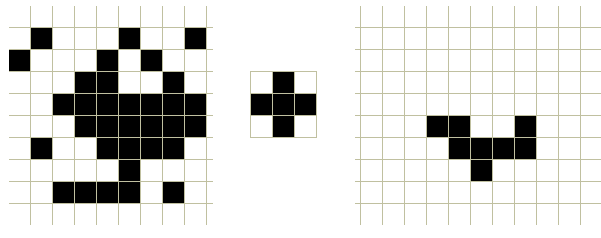
\includegraphics[width=15cm]{img/erode}
  \caption{Obraz binarny poddany procesowi erozji z zadanym elementem strukturalnym}
  \label{fig:erode}
\end{figure}
\subsubsection{Zamknięcie i otwarcie obrazu}
Operacje zamknięcia i otwarcia obrazu to złożenie dwóch wyżej wymienionych operacji (dylatacji oraz erozji) w odpowiedni sposób.
\begin{itemize}
\item zamknięcie obrazu definiowane jest w następujący sposób:
  \begin{gather*}
    A \bullet B = (A \oplus B) \ominus B,
  \end{gather*} 
czyli najpierw wykonywana jest operacja dylatacji obrazu, a następnie przekształcony obraz poddawany jest operacji erozji
\item otwarcie obrazu definiowane jest wzorem:
  \begin{gather*}
    A \circ B = (A \ominus B) \oplus B.
  \end{gather*}
W przypadku algorytmu otwarcia obrazu, w pierwszej kolejności wykonywana jest operacja erozji, a następnie operacja dylatacji obrazu.
\end{itemize}
Na rysunku~\ref{fig:open_close} przedstawiony został wynik działania obydwu algorytmów na tym samym obrazie, z tym samym elementem strukturalnym.
\begin{figure}
  \centering
  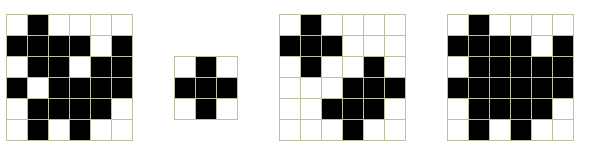
\includegraphics[width=15cm]{img/open-close}
  \caption{Obraz binarny poddany operacji otwarcia oraz zamknięcia obrazu, dla takiego samego elementu strukturalnego}
  \label{fig:open_close}
\end{figure}
\subsubsection{Transformata odległościowa}
Transformata odległościowa, inaczej zwana funkcją odległości, służy do wyznaczania minimalnej odległości punktu o wartości 1 od punktu o wartości 0. Dla punktów o wartości 0 automatycznie przypisywana jest wartość 0. \\
Tabela~\ref{tab:distance_transform} przedstawia wynik działania operacji na macierzy zawierającej obrazy binarne, natomiast rysunek~\ref{fig:distance_transform} prezentuje wynik działania tej samej operacji na obrazie. W celu podkreślenia wyniku operacji, obraz wyjściowy został poddany operacji normalizacji.

\begin{table}
\centering
\begin{minipage}[b]{80mm}
\centering
\begin{tabular}{|l|l|l|l|l|l|l|l|}
\hline
0&0&0&0&0&0&0&0 \\ \hline
0&1&1&1&1&1&1&0 \\ \hline
0&1&1&1&1&1&1&0 \\ \hline
0&1&1&1&1&1&1&0 \\ \hline
0&1&1&1&1&1&1&0 \\ \hline
0&1&1&1&1&1&1&0 \\ \hline
0&0&0&0&0&0&0&0 \\ \hline
\end{tabular}
\caption*{Binarny obraz wejściowy}
\end{minipage}
\begin{minipage}[b]{70mm}
\centering
\begin{tabular}{|l|l|l|l|l|l|l|l|}
\hline
0&0&0&0&0&0&0&0 \\ \hline
0&1&1&1&1&1&1&0 \\ \hline
0&1&2&2&2&2&1&0 \\ \hline
0&1&2&3&3&2&1&0 \\ \hline
0&1&2&2&2&2&1&0 \\ \hline
0&1&1&1&1&1&1&0 \\ \hline
0&0&0&0&0&0&0&0 \\ \hline
\end{tabular}
\caption*{Transformata odległościowa}
\end{minipage}
\caption{Transformacja odległościowa - macierz binarna} \label{tab:distance_transform} 
\end{table}

\begin{figure}
  \centering
  \begin{subfigure}[b]{0.45\textwidth}
    
\includegraphics[width=\textwidth]{img/distance-transform-before}
    \caption{Binarny obraz wejściowy}
    \label{fig:distance_transform_before}
  \end{subfigure}
  ~
  \begin{subfigure}[b]{0.45\textwidth}
    
\includegraphics[width=\textwidth]{img/distance-transform-after}
    \caption{Transformata odległościowa}
    \label{fig:distance_transform_after}
  \end{subfigure}
    \caption{Transformacja odległościowa - obraz binarny}
    \label{fig:distance_transform}
\end{figure}

\subsection{Operacje na histogramach}
Bardzo często podczas analizy obrazu pod kątem znajdowania segmentów, wykorzystywana jest analiza histogramu. W celu ułatwienia analizy, a także poprawy jej wyników, przed jej rozpoczęciem można zastosować niżej wymienione zabiegi.
\begin{figure}
  \centering
  \begin{subfigure}[b]{0.45\textwidth}
    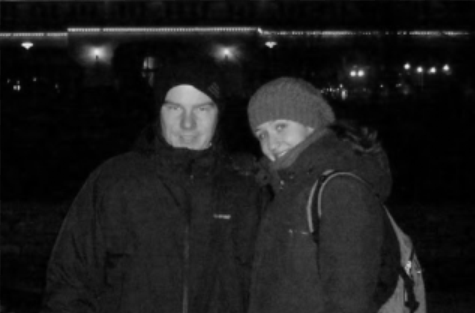
\includegraphics[width=\textwidth]{img/image-histogram}
    \label{fig:image_histogram}
  \end{subfigure}
  ~
  \begin{subfigure}[b]{0.45\textwidth}
    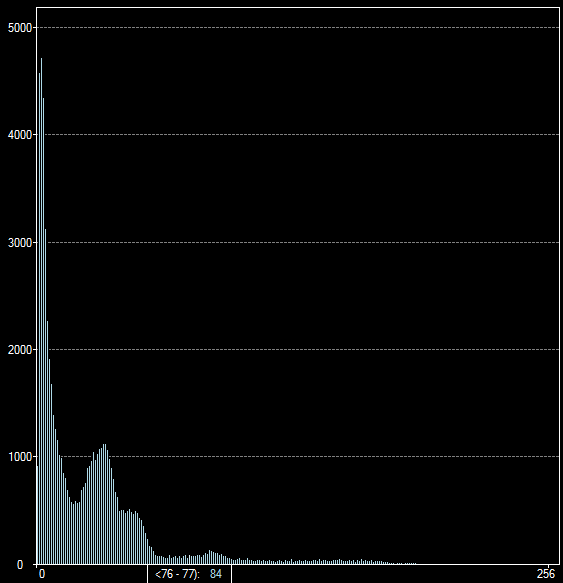
\includegraphics[width=\textwidth]{img/image-histogram-histogram}
    \label{fig:image_histogram_histogram}
  \end{subfigure}
  \caption{Jednokanałowy obraz oraz jego histogram}
  \label{fig:image_histogram_g}
\end{figure}
\textbf{Histogram obrazu} jest graficzną reprezentacją rozkładu częstości występowania danej wartości jasności w obrazie. Przykładowy obraz oraz jego histogram przedstawiony został na rysunku~\ref{fig:image_histogram_g}. Ponieważ obraz jest bardzo ciemny, większość wartości na histogramie jest bliska wartości 0 (ta wartość reprezentuje kolor czarny).\\
Jako $H$ będziemy oznaczali funkcję zwracającą wartość histogramu w podanym punkcie. Poprzez symbol $H_{max}$ oznaczać będziemy funkcję zwracającą największy indeks $i$ znajdujący się w histogramie, taki że $H(i) \neq 0$. Symbolem $H_{in}$ oznaczać będziemy histogram wejściowy, a symbolem $H_{out}$ histogram wyjściowy.\\

\subsubsection{Wyrównanie histogramu}
Metoda wyrównywania histogramu ma na celu zmianę kontrastu obrazu. Metoda ta wykorzystywany jest w przypadku, gdy zarówno tło, jak i pierwszy plan obrazu, są ciemne lub jasne. Wadą metody wyrównywania histogramu jest możliwe wzmocnienie zakłóceń występujących na obrazie, gdyż algorytm traktuje je jak sygnał opisujący prawidłowy obraz. Przed zastosowaniem tej metody, warto zatem zastosować jeden z algorytmów rozmycia obrazu, opisywany we wcześniejszej części tego rozdziału.\\
Metoda wyrównania histogramu sprowadza się do wyznaczenia tablicy LUT (\textit{ang. Lookup table}), na podstawie której wyznaczone zostaną wartości poszczególnych pikseli obrazu wejściowego. W celu wyznaczenia tablicy LUT, należy wyznaczyć dystrybuantę rozkładu prawdopodobieństwa dla wartości pikseli obrazu:
\begin{gather*}
  D(i) = \sum\limits_{j=0}^i p(j),
\end{gather*}
gdzie i jest wartością jasności występującą na obrazie, a p(j) jest prawdopodobieństwem wystąpienia wartości j w obrazie. Wykorzystując wyznaczone wartości dystrybuanty, możemy opisać tablicę LUT za pomocą wzoru:
\begin{gather*}
  LUT(i) = \frac{D(i)-D_0}{1-D_0} \cdot K,
\end{gather*}
gdzie i to wartość jasności składowej obrazu wejściowego, $D_0$ to pierwsza wartość dystrybuanty różna od zera, a K jest maksymalną wartością jasności występującym w obrazie wejściowym.\\
Rysunek~\ref{fig:equalize_histogram} przedstawia efekt działania operacji wyrównania histogramu na przykładowym obrazie.
\begin{figure}
  \centering
  \begin{subfigure}[b]{0.45\textwidth}
    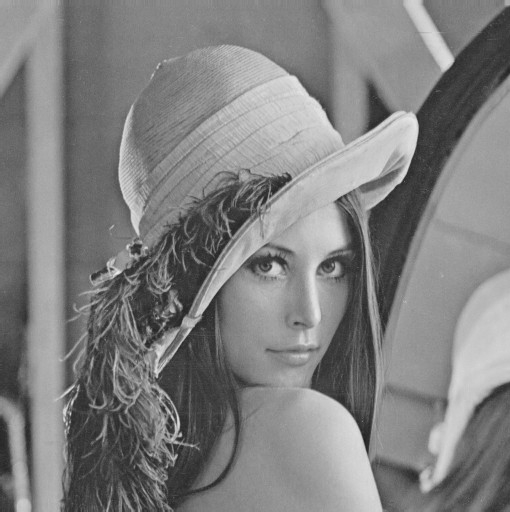
\includegraphics[width=\textwidth]{img/equalize-histogram-before}
    \caption{Obraz wejściowy dla operacji wyrównania histogramu}
    \label{fig:equalize_histogram_before}
  \end{subfigure}
  ~
  \begin{subfigure}[b]{0.45\textwidth}
    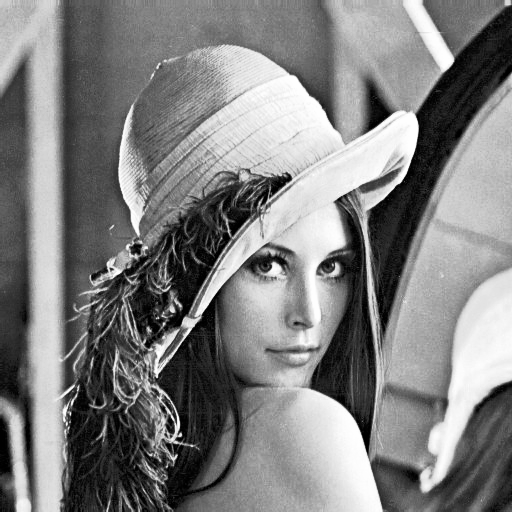
\includegraphics[width=\textwidth]{img/equalize-histogram-after}
    \caption{Obraz wyjściowy, poddany operacji wyrównania histogramu}
    \label{fig:equalize_histogram_after}
  \end{subfigure}
  ~
  \begin{subfigure}[b]{0.45\textwidth}
    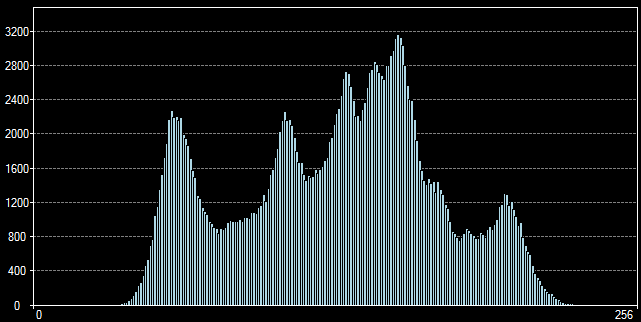
\includegraphics[width=\textwidth]{img/equalize-histogram-histogram-before}
    \caption{Histogram obrazu wejściowego}
    \label{fig:equalize_histogram_histogram_before}
  \end{subfigure}
  ~
  \begin{subfigure}[b]{0.45\textwidth}
    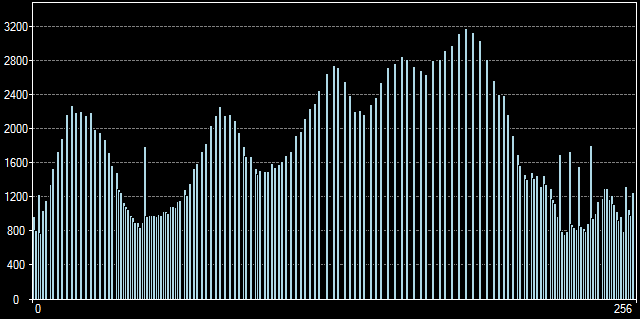
\includegraphics[width=\textwidth]{img/equalize-histogram-histogram-after}
    \caption{Histogram obrazu wyjściowego}
    \label{fig:equalize_histogram_histogram_after}
  \end{subfigure}
  \caption{Operacja wyrównania histogramu dla obrazu jednokanałowego}\label{fig:equalize_histogram}
\end{figure}

\subsubsection{Wygładzenie histogramu}
Często histogram obrazu zawiera w sobie nagłe skoki wartości, które utrudniają analizę histogramu, gdyż mogą reprezentować fałszywe ekstrema. Wygładzanie histogramu ma na celu usunięcie takich skoków, zachowując przy tym oryginalny kształt histogramu. Dla każdej wartości histogramu wejściowego \textit{$H_{in}$} należy zastosować następującą operację:
\begin{gather*}
  \forall_{i} \in \big< H_{in}(0), H_{in}(H_{max}(H_{in})) \big> :  H_{out}(i) = \frac{H_{in}(i-1) + H_{in}(i) + H_{in}(i+1)}{3}.
\end{gather*}
Przykład działania algorytmu wygładzania histogramu przedstawiony został na rysunku~\ref{fig:histogram_smooth}.
\begin{figure}
  \centering
  \begin{subfigure}[b]{0.45\textwidth}
    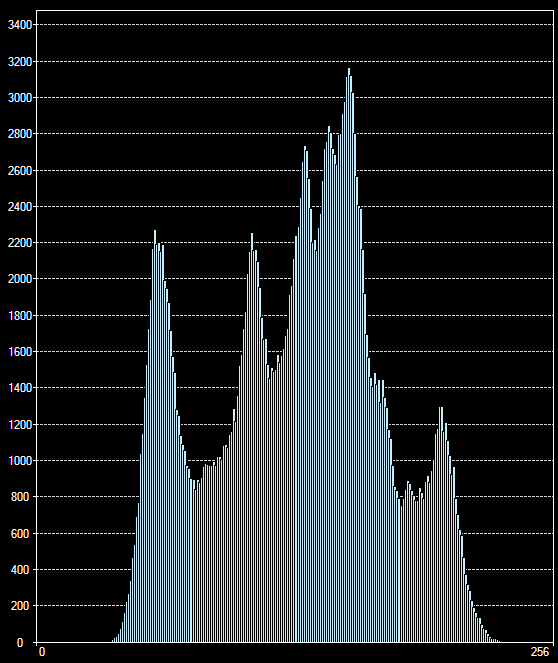
\includegraphics[width=\textwidth]{img/smooth-histogram-before}
    \caption{Obraz wejściowy dla operacji wygładzenia histogramu}
    \label{fig:equalize_histogram_before}
  \end{subfigure}
  ~
  \begin{subfigure}[b]{0.45\textwidth}
    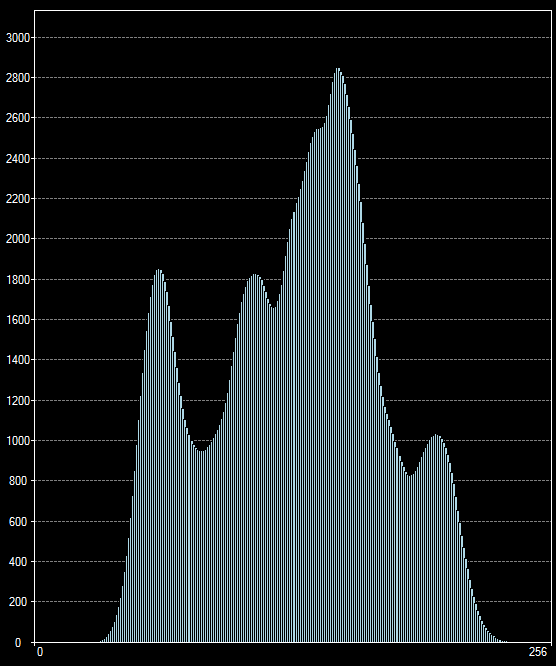
\includegraphics[width=\textwidth]{img/smooth-histogram-after}
    \caption{Obraz wyjściowy, poddany operacji wygładzenia histogramu}
    \label{fig:equalize_histogram_after}
  \end{subfigure}
  \caption{Operacja wygładzenia histogramu}\label{fig:histogram_smooth}
\end{figure}

\newpage
\section{Przegląd metod segmentacji obrazu}
\subsection{Wstęp}
Segmentacja obrazu jest procesem umożliwiającym podział obrazu na obszary, które pod względem zadanego kryterium różnią się miedzy sobą. W zależności od kryterium, podczas procesu segmentacji można wyodrębnić z obrazu obiekty posiadające określone kształty, kolory czy rozmiar. W wyniku segmentacji obrazu, uzyskujemy obraz, który nie zawiera zbędnych (z punktu widzenia dalszego przetwarzania) szczegółów.\\
Przykładem zastosowania metod segmentacji obrazów może być problem liczenia wbitych gwoździ do elementu na taśmie produkcyjnej. Obraz wejściowy (przedstawiony na rysunku~\ref{fig:gwozdzie_input}) ze względu na różnorodne tło i jasność elementów, trudno przeanalizować pod kątem liczenia obiektów. Natomiast ten sam obraz poddany operacji segmentacji (rysunek~\ref{fig:gwozdzie_output}) zawiera w sobie tylko i wyłącznie elementy, które są interesujące z punktu widzenia problemu jaki trzeba rozwiązać. Na podstawie koloru oraz kształtu możliwe było wyeliminowanie obiektów, które nie były istotne w danym zadaniu.

\begin{figure}
  \centering
  \begin{subfigure}[b]{0.48\textwidth}
    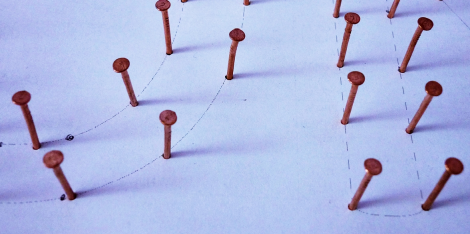
\includegraphics[width=\textwidth]{img/gwozdzie-input}
    \caption{Obraz wejściowy}
    \label{fig:gwozdzie_input}
  \end{subfigure}
  ~
  \begin{subfigure}[b]{0.48\textwidth}
    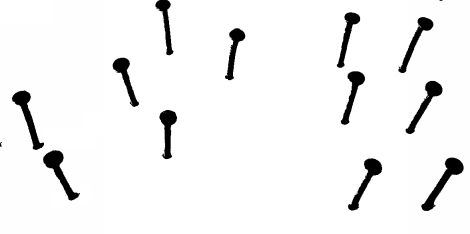
\includegraphics[width=\textwidth]{img/gwozdzie-output}
    \caption{Obraz po operacji segmentacji}
    \label{fig:gwozdzie_output}
  \end{subfigure}
  \caption{Przykład zastosowania metody segmentacji obrazu}\label{fig:gwozdzie}
\end{figure}

\subsection{Progowanie}
Najłatwiejszą metodą segmentacji obrazu jest metoda progowania, opisywana w podrozdziale \nameref{sssec:threshold}.

\subsection{Detekcja krawędzi}
Celem algorytmów detekcji krawędzi jest znalezienie na obrazie zbioru punktów, które reprezentują obrysy poszukiwanych elementów. 

\subsubsection{Algorytm Robertsa}
Algorytm Robertsa do wykrywania krawędzi w obrazie jest jednym z pierwszych algorytmów w swojej kategorii. Cechuje się szybkością działania oraz stosunkowo niską odpornością na szumy. Działanie algorytmu wymaga zastosowaniu dla każdego piksela obrazu dwóch masek:
\begin{gather*}
  M_x = \begin{matrix}
    \begin{bmatrix}
      +1 & 0 \\
      0 & -1
    \end{bmatrix}
    &
    M_y = \begin{bmatrix}
      0 & +1 \\
      -1 & 0
    \end{bmatrix}
  \end{matrix}
\end{gather*}
Zdefiniujemy funkcje pomocnicze $f_x$ oraz $f_y$:
\begin{gather*}
  f_x(x, y) = M_x * f^{(in)} \\
  f_x(x, y) = M_y * F^{(in)}.
\end{gather*}
Wartość jasności poszczególnych pikseli obrazu wyjściowego wyliczane są następującym wzorem:
\begin{gather*}
  f^{(out)}(x, y) = \sqrt{f_x^2(x, y)+f_{y}^2(x, y)}.
\end{gather*}
Kierunek gradientu może zostać wyznaczony ze wzoru:
\begin{gather*}
  \theta(x, y) = arctan(\frac{f_{y}(x, y)}{f_{x}(x, y)}).
\end{gather*}
\subsubsection{Sobel} \label{sssec:sobel}
Algorytmu Sobel jest bardzo podobny do przedstawionego wcześniej algorytmu Robertsa. W przypadku tego algorytmu, dane są dwie maski o następującej postaci:
\begin{gather*}
\begin{matrix}
  M_x = \begin{bmatrix}
    -1 & 0 & +1 \\
    -2 & 0 & +2 \\
    -1 & 0 & +1
  \end{bmatrix}
&
  M_y = \begin{bmatrix}
    -1 & -2 & -1 \\
    0 & 0 & 0 \\
    +1 & +2 & +1
  \end{bmatrix}
\end{matrix}
\end{gather*}
Zdefiniujemy dwie funkcje pomocnicze $f_x$ oraz $f_y$:
\begin{gather*}
  f_x  = M_x * f^{(in)}, \\
  f_y  = M_y * f^{(in)}.
\end{gather*}
Funkcję jasności obrazu wyjściowego możemy zdefiniować następująco:
\begin{gather*}
  f^{(out)}(x, y) = \sqrt{f_x^2(x, y)+f_{y}^2(x, y)}.
\end{gather*}
Algorytm jest znacznie bardziej odporny na szumy występujące na obrazie niż algorytm Robertsa. \\
Kierunek gradientu może zostać wyznaczony za pomocą wzoru:
\begin{gather*}
  \theta(x, y) = arctan(\frac{f_y(x, y)}{f_x(x, y)}).
\end{gather*}
\subsubsection{Algorytm Canny'ego}
Algorytm Canny'ego składa się z czterech podstawowych kroków.
\begin{enumerate}
\item Wygładzanie obrazu \\
  Celem tego kroku jest usunięcie z obrazu szumów mogących wystąpić na obrazie. Szumy mogą powodować detekcję fałszywych krawędzi, dlatego usunięcie ich przed faktycznym procesem wyszukiwania algorytmu powoduje poprawę jakości wyników algorytmu. W algorytmie Canny'ego do wygładzenia obrazu stosuje się filtr Gaussa. 
\item Znajdowanie gradientu \\
  Do znajdowania gradientu obrazu wykorzystywany jest operator sobela, opisywany w podrozdziale \nameref{sssec:sobel}.
\item Tłumienie sygnałów, które nie są maksymalne \\
  Po zastosowaniu operatora Sobel, krawędzie obrazu są rozmyte. W tym kroku następuje filtrowanie wszystkich lokalnych maksymalnych wartości w obrazie gradientowym, oraz usunięcie wartości nie-maksymalnych. Dla każdego piksela, kierunek gradientu zaokrąglany jest z dokładnością do 45 stopni, otrzymując w ten sposób 8 wartości kierunków. Dla każdego piksela pod uwagę brane są trzy wartości: wartość badanego piksela, najbliższy piksel wskazywany przez kierunek gradientu, oraz najbliższy piksel leżący w przeciwnym kierunku niż kierunek wskazywany przez gradient. Jeśli badany piksel ma wartość maksymalną spośród trzech podanych wartości, nie zostaje on usunięty. W przeciwnym razie, wartość piksela zostaje zastąpiona wartością zerową.
\item Podwójne progowanie(progowanie z histerezą)
  Pomimo zastosowania metody wygładzania w pierwszym etapie algorytmu, znalezienie niektórych krawędzi może być efektem zaszumionego obrazu. Dlatego w algorytmie Canny'ego stosuje się podwójne progowanie, z wartościami:\\
$T_{high}$ - wartość wyższego progu,\\
$T_{low}$ - wartość niższego progu,\\
będącymi w relacji:
\begin{gather*}
  T_{max} \geq T_{min}.
\end{gather*}
Piksele o wartościach większych niż $T_{high}$ klasyfikowane są jako \textit{krawędzie silne}. Piksele o wartościach pomiędzy $T_{low}$ i $T_{low}$ to tzw. \textit{krawędzie słabe}. Piksele o wartościach mniejszych niż $T_{min}$ są usuwane z obrazu.

\end{enumerate}

\subsection{Algorytmy wykorzystujące histogram}
Algorytmy wykorzystujące analizę histogramu obrazu cechuje szybkość działania, ponieważ budowa histogramu wymaga tylko jednej iteracji przez wszystkie piksele w obrazie. Istnieje kilka technik segmentacji obrazu w oparciu o analizę histogramu. \\
Przed wykonaniem jednego z niżej omawianych algorytmów, w celu poprawy rezultatów, należy zastosować operację wyrównania histogramu, oraz operację wygładzenia histogramu.

\subsubsection{Wyszukiwanie szczytów histogramu}
Wyszukiwanie szczytów histogramu wykorzystywane jest do separacji tła od obiektu pierwszoplanowego. Po wyznaczeniu histogramu, wyszukiwane zostają dwa maksimum lokalne, posiadające największe wartości (są to tzw. wartości szczytowe). Następnie na podstawie tych wartości wyznaczana jest progowa wartość, służąca do klasyfikacji pikseli na obrazie:
\begin{gather*}
  T = \frac{p_1 + p_2}{2},
\end{gather*}
gdzie $p_1$ jest pierwszą wartością szczytową w histogramie, a $p_2$ jest drugą wartością szczytową w histogramie. \\
W rzeczywistych przypadkach bardzo często występuje sytuacja, w której piksele tła oraz piksele obiektu pierwszoplanowego nie mają takich samych wartości dla całego obiektu, ale przyjmują wiele wartości oscylujących wokół jednej z nich. Przykład takiego obrazu został pokazany na rysunku~\ref{fig:histogram_peaks}. Histogram zawiera widoczne trzy skupiska wartości (na pozycjach: 8, 18 oraz 44), natomiast obydwie największe wartości szczytowe w histogramie należą do jednego skupiska. Aby wyeliminować ten problem, należy zdefiniować minimalną odległość pomiędzy szczytami histogramu. Jeśli drugi szczyt będzie znajdował się zbyt blisko pierwszego, należy go odrzucić, i rozpocząć poszukiwanie kolejnego szczytu. Nie uwzględniając minimalnego odstępu pomiędzy szczytami, do wyznaczenia progu zostały by wybrane liczby 8 oraz 18, ponieważ są to dwie największe wartości w histogramie. Obydwie te wartości reprezentują tło, przez co segmentacja się nie powiodła (co można zobaczyć na rysunku~\ref{fig:histogram_peaks_bad}. Jeśli założymy, że szczyty nie mogą znajdować się od siebie bliżej niż wartość $\frac{1}{3}$ szerokości histogramu, do wyznaczenia progu zostanie użyta wartość 8 oraz 44. Wynikiem segmentacji natomiast będzie obraz przedstawiony na rysunku~\ref{fig:histogram_peaks_good}. Zwykle wartość minimalnej odległości pomiędzy szczytami dobiera się na podstawie przeprowadzonych wcześniej badań na danych testowych.
\begin{figure}
  \centering
  \begin{subfigure}[b]{0.7\textwidth}
    
\includegraphics[width=\textwidth]{img/histogram-peaks-input}
    \caption{Obraz wejściowy}
    \label{fig:histogram_peaks_input}
  \end{subfigure}
  ~
  \begin{subfigure}[b]{0.7\textwidth}
    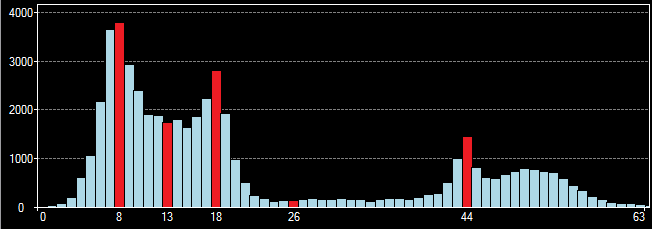
\includegraphics[width=\textwidth]{img/histogram-peaks-histogram}
    \caption{Histogram obrazu wejściowego}
    \label{fig:histogram_peaks_histogram}
  \end{subfigure}
  ~
  \begin{subfigure}[b]{0.45\textwidth}
    
\includegraphics[width=\textwidth]{img/histogram-peaks-bad}
    \caption{Obraz po operacji progowania, wartość progu: 13}
    \label{fig:histogram_peaks_bad}
  \end{subfigure}
  ~
  \begin{subfigure}[b]{0.45\textwidth}
    
\includegraphics[width=\textwidth]{img/histogram-peaks-good}
    \caption{Obraz po operacji progowania, wartość progu: 26}
    \label{fig:histogram_peaks_good}
  \end{subfigure}
  \caption{Progowanie przez wyszukiwanie szczytów histogramu}\label{fig:histogram_peaks}
\end{figure}

\subsubsection{Wyszukiwanie minimum histogramu}
Metoda wyszukiwania minimum histogramu jest bardzo podobna do metody omawianej w poprzednim podpunkcie. Na początku wyszukiwane są dwie wartości szczytowe, które powinny być odległe od siebie o pewną ustaloną wartość. Jednak w przeciwieństwie do omawianego wcześniej algorytmu, jako wartość progową przyjmuje się najmniejszą wartość pomiędzy dwoma szczytami w histogramie. \\
Rysunek~\ref{fig:histogram_valleys} przedstawia histogram pewnego obrazu. Stosując metodę wyszukiwania szczytów histogramu, jako wartość progowa wybralibyśmy wartość 102 (szczyty histogramów znajdują się na pozycjach 48 i 155). Stosując omawianą w tym podpunkcie metodę, jako wartość progowa zostanie wybrana wartość 129, która jest minimalną wartością znajdującą się pomiędzy szczytami histogramu.

\begin{figure}
  \centering
  \begin{subfigure}[b]{0.7\textwidth}
    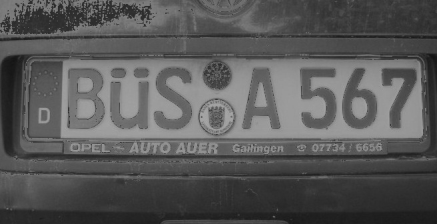
\includegraphics[width=\textwidth]{img/histogram-valleys-input}
    \caption{Obraz wejściowy}
    \label{fig:histogram_valleys_input}
  \end{subfigure}
  ~
  \begin{subfigure}[b]{0.7\textwidth}
    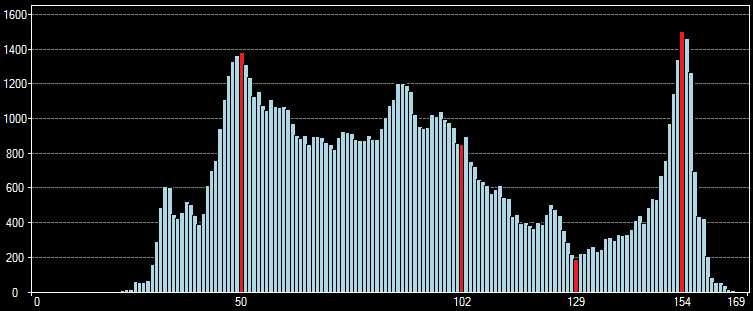
\includegraphics[width=\textwidth]{img/histogram-valleys-histogram}
    \caption{Histogram obrazu wejściowego}
    \label{fig:histogram_valleys_histogram}
  \end{subfigure}
  ~
  \begin{subfigure}[b]{0.45\textwidth}
    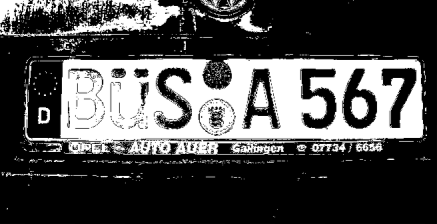
\includegraphics[width=\textwidth]{img/histogram-valleys-bad}
    \caption{Obraz po operacji progowania, wartość progu: 102}
    \label{fig:histogram_valleys_bad}
  \end{subfigure}
  ~
  \begin{subfigure}[b]{0.45\textwidth}
    
\includegraphics[width=\textwidth]{img/histogram-valleys-good}
    \caption{Obraz po operacji progowania, wartość progu: 129}
    \label{fig:hitogram_valleys_good}
  \end{subfigure}
  \caption{Progowanie przez wyszukiwanie minimum pomiędzy szczytami histogramu}\label{fig:histogram_valleys}
\end{figure}
\subsection{Segmentacja przez rozrost obszarów}
Metoda segmentacji przez rozrost obszarów polega na wyszukiwanie na obrazie elementów o podobnej jasności. Algorytm rozpoczyna działanie od punktów startowych, które powinny zostać podane jako parametr algorytmu. Algorytm można opisać w następujący sposób:
\begin{enumerate}
  \item Nadaj każdemu punktowi startowemu etykietę.
  \item Dodaj punkty startowe do kolejki.
  \item Jeśli kolejka jest pusta, zakończ algorytm.
  \item Pobierz punkt z kolejki, a następnie sprawdź wszystkie punkty znajdujące się w sąsiedztwie pod względem podobieństwa. Jeśli sąsiedni punkt spełnia kryterium podobieństwa, oznacz go etykietą punktu pobranego z kolejki, a następnie umieść punkt w kolejce.
  \item Przejdź do kroku 3.
\end{enumerate}
Wynikiem algorytmu będzie zbiór punktów oznaczonych etykietami. Punkty oznaczone tą samą etykietą reprezentują pojedynczy obszar znaleziony na obrazie.

Podczas projektowania metody segmentacji przez rozrost, należy, biorąc pod uwagę warunki działania algorytmu, rozważyć dwa problemy:
\begin{itemize}
  \item wybór punktów startowych,
  \item wybór kryterium podobieństwa.
\end{itemize}
W celu rozwiązania pierwszego problemu, można zastosować jedną z wcześniej omawianych metod segmentacji (np. szybki algorytm progowania), a następnie wybrać punkty oddalone od siebie o zadaną wartość. \\
Kryterium podobieństwa może zostać określone na dwa sposoby, w zależności od problemu, do rozwiązywania którego został zaprojektowany algorytm:
\begin{enumerate}
  \item dla obrazów w których różnica jasności w ramach jednego obszaru może być bardzo duża, należy zastosować kryterium 
    \begin{gather*}
      |f^{(in)}(p_x, p_y) - f^{(in)}(n_x, n_y)| < \varepsilon,
    \end{gather*}
    gdzie $p_x$ oraz $p_y$ to współrzędne aktualnie przetwarzanego punktu, $n_x$ i $n_y$ to współrzędne aktualnie przetwarzanego sąsiada, a $\varepsilon$ to maksymalna różnica jasności pomiędzy sąsiednimi punktami, taka, że dwa punkty uznawane są za przynależne do tego samego obiektu. Stosując powyższe kryterium mamy pewność, że obiekt ze zmiennym natężeniem oświetlenia zostanie sklasyfikowany jako jeden obszar. Stosowanie tego kryterium może jednak spowodować, że do obszaru zostaną zaklasyfikowane elementy tła.
    \item dla obrazów o stałym oświetleniu, stosuje się kryterium
      \begin{gather*}
        |f^{(in)}(seed_x, seed_y) - f^{(in)}(n_x, n_y)| < \varepsilon
      \end{gather*}
      gdzie $seed_x$ i $seed_y$ to współrzędne punktu wejściowego. Stosując powyższe kryterium mamy pewność, że obiekt ze zmiennym natężeniem oświetlenia zostanie sklasyfikowany jako jeden obszar. Stosowanie tego kryterium może jednak spowodować, że do obszaru zostaną zaklasyfikowane elementy tła.
\end{enumerate}
Na rysunku~\ref{fig:region_growing} przedstawiony został wynik operacji segmentacji obrazu przez rozrost obszarów stosując dwa różne kryteria.
\begin{figure}
  \centering
  \begin{subfigure}[b]{0.45\textwidth}
    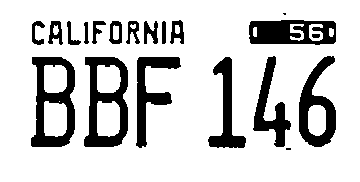
\includegraphics[width=\textwidth]{img/region-growing-relative}
    \caption{Obraz wynikowy dla kryterium 1)}
    \label{fig:region_growing_relative}
  \end{subfigure}
  ~
  \begin{subfigure}[b]{0.45\textwidth}
    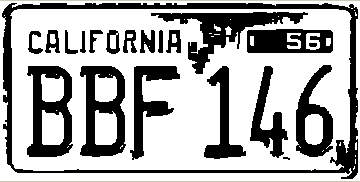
\includegraphics[width=\textwidth]{img/region-growing-absolute}
    \caption{Obraz wynikowy dla kryterium 2)}
    \label{fig:region_growing_absolute}
  \end{subfigure}
  \caption{Porównanie wyników uruchomienia algorytmu rozrostu obszarów z zastosowaniem różnych kryterium}
    \label{fig:region_growing}
\end{figure}

\subsection{Segmentacja przy użyciu rzutu jasności} \label{ssec:rzut_jasnosci}
Algorytm rzutu jasności bardzo dobrze sprawdza się w lokalizacji obiektów na obrazie, kiedy natężenie koloru obiektu znacząco różni się od koloru tła, a ponadto, obiekty zajmują znaczącą część powierzchni obrazu. Obraz rozpatrywany jest zarówno w poziomie, jak i w pionie. Dla każdego wiersza(kolumny) w obrazie, sumuje się wszystkie wartości pikseli należące dla danego wiersza(kolumny), otrzymując tablicę wartości:
\begin{gather*}
  G_x[i] = \sum\limits_{i=1}^M f^{(in)}(i, j) \; dla \; i = 0,1,2,...,M, \\
  G_y[j] = \sum\limits_{j=1}^N f^{(in)}(i, j) \; dla \; j = 0,1,2,...,N,
\end{gather*} gdzie $G_x$ oraz $G_y$ to tablice rzutu jasności. Analizując tablice rzutu jasności można zauważyć, że w miejscach na obrazie, gdzie występują obiekty, wartości w tablicy przyjmują wartości znacznie większe w przypadku, gdy kolor tła jest ciemniejszy od obiektu, lub znacznie mniejsze, w przypadku gdy kolor tła jest jaśniejszy od obiektu. Na podstawie tych informacji możliwe jest zlokalizowanie obiektów na obrazie. Rysunek~\ref{fig:rzut_jasnosci} przedstawia użycie metody segmentacji przy użyciu rzutu jasności dla przykładowej tablicy rejestracyjnej. Tablice rzutu jasności przedstawione zostały w postaci histogramu. W miejscach, gdzie pojawiają się na obrazie litery, wartości histogramu są mniejsze.

\begin{figure}
  \centering
  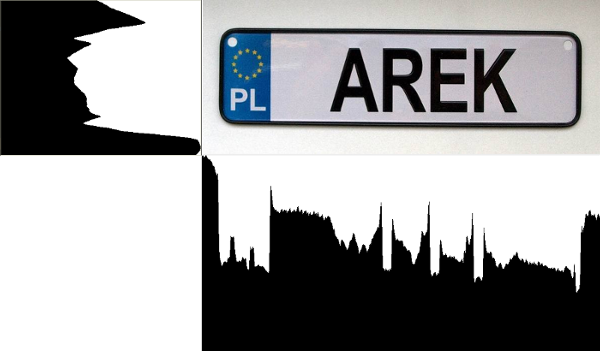
\includegraphics[width=15cm]{img/rzut-jasnosci}
  \caption{Histogramy dla obrazu wygenerowane przez algorytm rzutu jasności dla przykładowego obrazu}
  \label{fig:rzut_jasnosci}
\end{figure}
\subsection{Metoda Sauvola i Pietikainena}
Algorytm polega na znalezieniu progu dla każdego piksela, analizując jego najbliższe otoczenia. Otoczenie rozumiemy przez zbiór pikseli które znajdują się w zdefiniowanym obszarze, a piksel, dla którego w danym momencie wyznaczana jest wartość progu, znajduje się na środku tego obszaru. Wartość progu wyznaczana jest według wzoru:
\begin{gather*}
  T(x, y) = \mu(x, y)\Big[1+k\big(\frac{\sigma(x, y)}{R} - 1\big)\Big], \quad k > 0,
\end{gather*}
gdzie:
T(x, y) - wartość progu dla piksela o współrzędnych (x, y),\\
$\mu$(x, y) - średnia wartości pikseli w zadanym otoczeniu piksela,\\
$\sigma(x, y)$ - odchylenie standardowe w zadanym otoczeniu piksela,\\
R - maksymalna wartość odchylenia standardowego(dla obrazu 8-bitowego jest to wartość 128),\\
k - parametr algorytmu. \\
\subsection{Segmentacja wododziałowa}
Algorytm segmentacji wododziałowej polega na odnajdowaniu na obrazie krawędzi, będących granicami szukanych segmentów. Segmentacja wododziałowa wzorowana jest na naturalnym procesie hydrologicznym, polegającym na tworzeniu się zlewisk w lokalnie najniżej położonych obszarach geograficznych. \\
\subsubsection{Podstawowe pojęcia}
Algorytm zostanie opisany używając terminologii występującej w geografii. Poniżej znajduje się rozwinięcie podstawowych pojęć:
\begin{itemize}
  \item zlewisko - obszar, z którego wszystkie wody spływają do większego zbiornika wodnego,
  \item wododział - linia oddzielająca od siebie tereny zlewisk.
\end{itemize}
Na rysunku~\ref{fig:watershed_graphic} graficznie przedstawione zostały omawiane wyżej pojęcia.
\begin{figure}
  \centering
  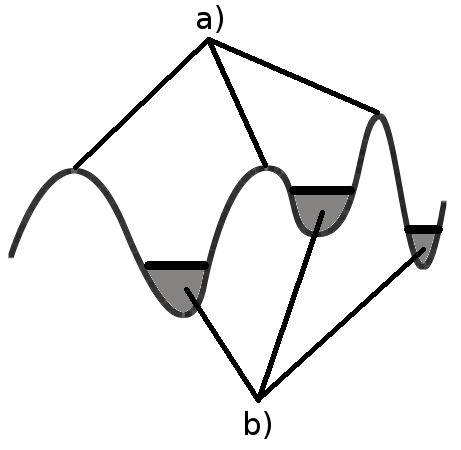
\includegraphics[width=9cm]{img/watershed-graphic}
  \caption{Graficzna reprezentacja a) wododziałów, b) zlewisk }
  \label{fig:watershed_graphic}
\end{figure}
W kontekście przetwarzania obrazów, wysokość terenu reprezentowana jest przez funkcję amplitudy gradientu obrazu lub funkcję intensywności obrazu, natomiast wododziały to ekstrema lokalne tych funkcji.
\subsubsection{Algorytm segmentacji wododziałowej}
Omawiany niżej algorytm został zaproponowany przez F. Meyera.
\begin{enumerate}
  \item wybierane są punkty startowe, będące również etykietami poszczególnych segmentów obrazu,
  \item sąsiadujące z wybranymi w kroku 1) punktami piksele umieszczane są w kolejce priorytetowej, gdzie priorytet stanowi jasność piksela,
  \item z kolejki pobierany jest piksel o najwyższym priorytecie. Jeśli wszystkie piksele w jego sąsiedztwie, którym została przypisana etykieta, mają tę samą etykietę, wtedy przetwarzany piksel również otrzymuje tę etykietę,
  \item wszystkie sąsiadujące piksele, które nie zostały oznaczone etykietą, umieszczane są w kolejce,
  \item jeśli kolejka nie jest pusta, powtarzany jest punkt 3). W przeciwnym razie algorytm zostaje zakończony.
\end{enumerate}
Piksele, które nie zostały oznaczone, reprezentują wododziały. Piksele oznaczone tą samą etykietą, należą do tego samego zlewiska, czyli tworzą ten sam segment.

\newpage
\section{Algorytm rozpoznawania znaków}
Segmentacja obrazu prowadzi do wyodrębnienia z obrazu żądanych obiektów. Zwykle jest ona pierwszym etapem analizy całego obrazu. Odnalezione obiekty bardzo często poddawane są analizie w celu identyfikacji lub podjęcia decyzji.
\paragraph{}
W przypadku problemu rozpoznawania znaków, zadaniem algorytmu segmentacji jest określenie lokalizacji każdego znaku oraz binaryzacja fragmentów obrazu zawierającego tekst. Kolejnym krokiem jest dostarczenie serii wykadrowanych obrazów binarnych zawierających pojedyncze znaki do algorytmu rozpoznawania znaków. Zadaniem algorytmu rozpoznawania znaków jest określenie, jaki znak tekstu znajduje się na zadanym obrazie.
\paragraph{}
Poniżej zostanie opisanych kilka algorytmów rozpoznawania znaków.
\subsection{Cechy geometryczne}
Zestaw cech geometrycznych jest unikalny dla każdego znaku, dlatego sprawdzając odpowiednie warunki, można określić jego dokładne znaczenie. Poniżej znajduje się lista cech geometrycznych, które mogą być brane pod uwagę podczas rozpoznawania znaków.
\begin{itemize}
  \item wysokość oraz szerokość prostokąta otaczającego znak
  \item stosunek liczby punktów należących do znaku do liczby punktów stanowiących tło
  \item stosunek liczby punktów należących do znaku i znajdujących się w górnej połówce obrazu, do liczby punktów należących do znaku i znajdujących się w dolnej połówce obrazu
    \item stosunek liczby punktów należących do znaku i znajdujących się w lewej połówce  obrazu, do liczby punktów należących do znaku i znajdujących się w prawej połówce obrazu
    \item liczba pionowych oraz poziomych krawędzi znaku
\end{itemize}
\subsection{Rzut jasności obiektu}
Metoda rzutu jasności obiektu została opisana w podrozdziale~\ref{ssection:rzut_jasnosci}. W pierwszej kolejności należy przeskalować obraz do rozmiarów obrazu wzorcowego, a następnie wykonać algorytm rzutu jasności zarówno w pionie, jak i w poziomie. Otrzymane rzuty zostają następnie poddane analizie podobieństwa z rzutami wykonanymi dla znaków wzorcowych. Analiza podobieństwa polega na porównaniu kształtu otrzymanych rzutów jasności. \\
Na rysunku~\ref{fig:rzut_jasnosci_ocr} przedstawione zostały wzorce kilku znaków, oraz przykładowy obraz wejściowy.

\begin{figure}
  \centering
  \begin{subfigure}[b]{0.42\textwidth}
    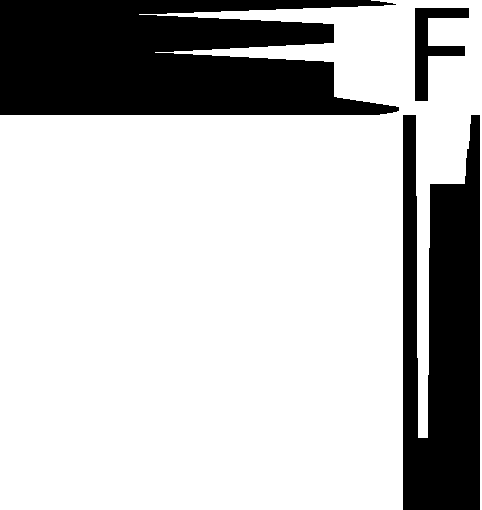
\includegraphics[width=\textwidth]{img/rzut-wzorzec-F}
    \caption{Wzorzec dla litery F}
    \label{fig:rzut_wzorzec_F}
  \end{subfigure}
  ~
  \begin{subfigure}[b]{0.42\textwidth}
    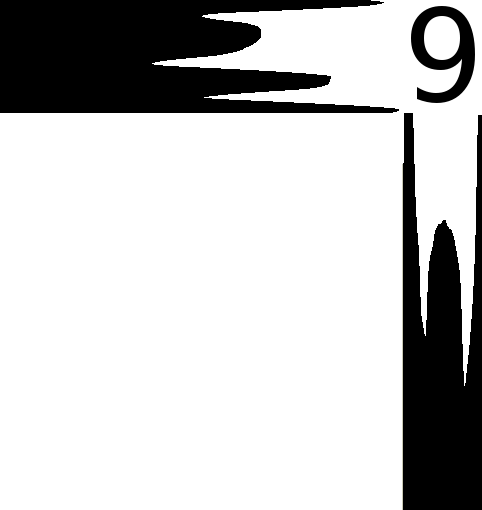
\includegraphics[width=\textwidth]{img/rzut-wzorzec-9}
    \caption{Wzorzec dla cyfry 9}
    \label{fig:rzut_wzorzec_9}
  \end{subfigure}
  \begin{subfigure}[b]{0.44\textwidth}
    
\includegraphics[width=\textwidth]{img/rzut-in-9}
    \caption{Obraz wejściowy, zawierający cyfrę 9}
    \label{fig:rzut_in_9}
  \end{subfigure}
  \caption{Porównanie rzutu jasności dla wybranych znaków}
    \label{fig:rzut_jasnosci_ocr}
\end{figure}

\subsection{Sztuczne sieci neuronowe}
Sztuczne sieci neuronowe(SSN) to struktury tworzone na podobieństwo biologicznych sieci neuronowych. SSN mają zdolność do uogólniania zdobytej wiedzy. Podobnie jak w przypadku biologicznych, w sztucznych sieciach neuronowych podstawowym elementem są neurony, które połączone są miedzy sobą za pomocą synaps. Każda synapsa posiada parametr zwany wagą, który jest modyfikowany w poszczególnych fazach uczenia sieci neuronowej. Sieci neuronowe zorganizowane są w strukturze wielowarstwowej:
\begin{itemize}
  \item warstwa wejściowa,
  \item warstwy ukryte,
  \item warstwa wyjściowa
\end{itemize}. W zależności od złożoności problemu, sieć neuronowa może zawierać różną liczbę neuronów w każdej warstwie, oraz różną liczbę warstw ukrytych. Przykład SSN można znaleźć na rysunku~\ref{fig:ssn_example}. Wartość wyjściowa neuronu wyznaczana jest na podstawie sygnałów wejściowych oraz funkcji aktywacji. Dla każdego neuronu wartość wyjściowa wyznaczana jest za pomocą wzoru:
\begin{gather*}
  y = g(\sum_{i=1}^{N}w_ix_i+w_0)
\end{gather*}, gdzie:
\begin{itemize}
  \item g - funkcja aktywacji,
  \item N - liczba wejść poprzedniej warstwy,
  \item $w_i$ - waga synapsy i-tego sygnału,
  \item $x_i$ - wartość i-tego sygnału
\end{itemize}. W zależności od wybranego algorytmu, sieć poddawana jest procesowi uczenia, podczas którego wartości wag $w_i$ są korygowane.\\
Jako zestaw uczący, a następnie zestaw testowy, podawane mogą być obrazy ze znakami. Po wykonaniu procesu uczenia, sieć neuronowa powinna mieć zdolność do dopasowania obrazu do najlepszego wyuczonego wzorca. 
\begin{figure}
  \centering
  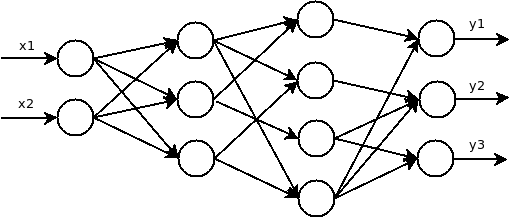
\includegraphics[width=10cm]{img/ssn-example}
  \caption{Przykładowa sieć neuronowa, zawierająca dwa neurony w warstwie wejściowej, dwie warstwy ukryte, oraz warstwę wejściową zawierającą trzy neurony.}
  \label{fig:ssn_example}
\end{figure}

\newpage
\section{Segmentacja obrazów tablic rejestracyjnych}
Podczas pracy nad algorytmami segmentacji obrazu, przede wszystkim skupiłem się na problemie segmentacji tablic rejestracyjnych. Segmentacja jest kluczowym elementem procesu identyfikacji tablicy rejestracyjnej.\\
Algorytmy rozpoznawania tablic rejestracyjnych wykorzystywane są bardzo często w rozwiązaniach przemysłowych, przez co wymagana jest wysoka jakość zwracanych wyników.\\
Ze względu na różnorodność formatów tablic rejestracyjnych, jakie mogą wystąpić, oraz dodatkowych utrudnień związanych z niedoskonałością środowiska, w którym wykonywany jest obraz, problem segmentacji tablic rejestracyjnych nie jest problemem łatwym do rozwiązania.
\paragraph{}
Obrazy tablic rejestracyjnych, ze względu na warunki w jakich są wykonywane, nie zawierają jedynie tekstu, który jest łatwy do analizy. Obrazy często zawierają artefakty, tablice mogą być zanieczyszczone, lub ze względu na warunki atmosferyczne, obraz może być niejednolicie oświetlony. Opisałem problemy, z jakimi spotkałem się, analizując zestaw danych testowych, wraz z proponowanymi przeze mnie możliwościami rozwiązania problemów.\\
W tym rozdziale będę stosował formę zapisu wzorów matematycznych stosowaną w języku programowania C++.
\subsection{Różne kolory tablic rejestracyjnych}\label{ssec:different_backgrounds}
Algorytmy segmentacji tablic rejestracyjnych, które zaprezentuję w dalszej części pracy, wymagają, aby tło tablic rejestracyjnych było jaśniejsze od tekstu. Dlatego opracowałem algorytm, który wykrywa odwrotną sytuację (kiedy tło jest ciemniejsze od znaków), i w razie potrzeby, odwróci kolory obrazu.\\
Pierwszym pomysłem było zastosowanie lokalnego progowania, a następnie policzenie czarnych oraz białych pikseli, aby w zależności od tego, który kolor występuje częściej, określić tło tablicy rejestracyjnej. Metoda ta okazała się w większości przypadków skuteczna. Algorytm nie zwracał jednak poprawnych rezultatów w przypadku, gdy obraz tablicy rejestracyjnej wykonany był pod kątem, i nie można było wykadrować obrazu w taki sposób, aby pozbyć się niepożądanych pikseli. Rysunek~\ref{fig:detect_bg_bad} przedstawia ten problem. Tablica rejestracyjna zajmuje większą część obrazu, jednak pomimo tego, została sklasyfikowana przez algorytm jako tablica z czarnym tłem. Wynika to z faktu, iż na tablicy pozostały znaki, które również zajmują znaczącą powierzchnię obrazu. Następnie spróbowałem zastosować operację zamknięcia regionu, która poprawnie usunęła znaki z obrazu. Nie zadziałała jednak w przypadku białych znaków na czarnym tle. \\
Zamiast operacji morfologicznej, zastosowałem rozmycie medianowe, które dało poprawny efekt zarówno dla czarnych znaków na białym tle, jak również dla białych znaków na czarnym tle. Na rysunku~\ref{fig:detect_bg_ok} przedstawiony został wynik eksperymentu dla obrazu wejściowego przedstawionego na rysunku~\ref{fig:detect_bg_bad}. Jak można zauważyć, algorytm usunął zawartość tablicy rejestracyjnej, pozostawiając jedynie tło tablicy. Zwiększyło to tym samym ilość znaków tła, przez co algorytm poprawnie rozpoznał kolor tła jako biały.

\begin{figure}
  \centering
  \begin{subfigure}[b]{0.45\textwidth}
    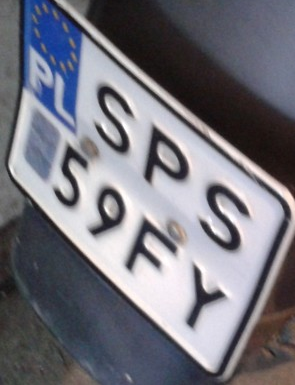
\includegraphics[width=\textwidth]{img/detect-bg-bad-input}
    \label{fig:detect_bg_bad_input}
    \caption{}
  \end{subfigure}
  ~
  \begin{subfigure}[b]{0.45\textwidth}
    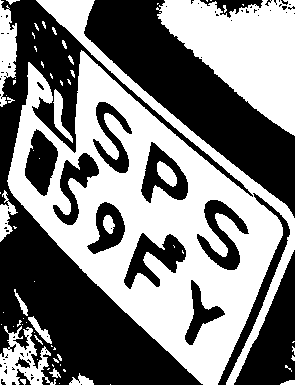
\includegraphics[width=\textwidth]{img/detect-bg-bad-output}
    \label{fig:detect_bg_bad_output}
    \caption{}
  \end{subfigure}
  \caption{Operacja progowania lokalnego}
  \label{fig:detect_bg_bad}
\end{figure}

\begin{figure}
  \centering
  
\includegraphics[width=7cm]{img/detect-bg-ok-output}
  \caption{Obraz po wykonaniu operacji usuwania znaków przez rozmycie medianowe}
  \label{fig:detect_bg_ok}
\end{figure}

\subsection{Obrazy wykonane pod różnymi kątami}
Bardzo często zdarza się, że obraz tablicy rejestracyjnej nie został wykonany idealnie na wprost obiektu. Efektem tego mogą być obrazy, których numery rejestracyjne są pochylone, co może powodować ich niepoprawną lokalizację oraz identyfikację. \\
\textbf{Algorytm detekcji kąta obrotu}. W tym szczególnym przypadku udało mi się rozwiązać ten problem w niżej opisany sposób. Wymaga on założenia, że tło tablicy rejestracyjnej jest jaśniejsze od pozostałych obiektów znajdujących się na obrazie, natomiast jeśli wcześniej zostanie zastosowany algorytm unifikacji tła tablicy rejestracyjnej, omawiany w poprzednim podrozdziale, warunek ten będzie spełniony.
\paragraph{}
Na początku, obraz poddajemy działaniu jednego z algorytmów progowania. Wynik tego progowania nie musi dawać nam bardzo dobrego rezultatu, jeśli chodzi o rozdzielenie znaków od tła, ważne jest tylko, aby wyraźnie zostało zaznaczone tło. Można zastosować jeden z algorytmów progowania dynamicznego, lub progowania globalnego z wysokim progiem. Po zastosowaniu algorytmu progowania, znajdujemy największy spójny biały obszar, a następnie wyznaczamy najmniejszy prostokąt otaczający ten obszar. Kąt, pod jakim znajduje się prostokąt, jest kątem, o jaki obrócony został obraz podczas jego tworzenia.\\
Poszczególne kroki działania algorytmu zostały przedstawione na rysunku~\ref{fig:detect_image_angle}.

\begin{figure}
  \centering
  \begin{subfigure}[b]{0.45\textwidth}
    \includegraphics[width=\textwidth]{img/detect-image-angle-input}
    \label{fig:rzut_liczba_linii_jeden}
    \caption{}
  \end{subfigure}
  ~
  \begin{subfigure}[b]{0.45\textwidth}
    \includegraphics[width=\textwidth]{img/detect-image-angle-threshold}
    \label{fig:rzut_liczba_linii_dwa}
    \caption{}
  \end{subfigure}
  ~
  \begin{subfigure}[b]{0.45\textwidth}
    \includegraphics[width=\textwidth]{img/detect-image-angle-output}
    \label{fig:rzut_liczba_linii_dwa}
    \caption{}
  \end{subfigure}
  \caption{Wyniki operacji poszczególnych kroków algorytmu rotacji obrazu: a) obraz wejściowy, b) progowanie i znajdowanie prostokąta obejmującego, c) obraz wynikowy.}
  \label{fig:detect_image_angle}
\end{figure}


\subsection{Różne formaty zapisu danych}\label{ssec:different_formats}
Numer rejestracyjny pojazdu może być zapisany jako jedna, lub jako dwie linie tekstu. Założeniem algorytmu rozpoznawania tablic rejestracyjnych jest możliwość rozpoznania obydwóch formatów zapisu, dlatego przed przystąpieniem do dalszej analizy, należy określić liczbę linii tekstu. Znajomość liczby linii jest przydatna podczas oceny ostatecznego rozwiązania segmentacji obrazu, ponieważ znana jest wtedy przybliżona lokalizacja liter. Poniżej przedstawiam propozycję dwóch rozwiązań problemu detekcji liczby linii wykorzystanych do zapisu numeru rejestracyjnego.
\paragraph{Metoda rzutu jasności obrazu.} Algorytm rzutu jasności obrazu opisywany był na stronie~\pageref{ssec:rzut_jasnosci}. Zauważyłem, że algorytm ten może również zostać wykorzystany do określenia liczby linii tekstu, wykorzystując do tego tylko poziomy rzut jasności dla obrazu. Na rysunku~\ref{fig:rzut_liczba_linii} zamieszczone zostały dwa obrazy przedstawiające rzuty jasności dla tablicy rejestracyjnej zawierającej jedną, oraz dwie linie tekstu. Można zauważyć, że w miejscach, gdzie nie znajduje się tekst, wykres rzutu jasności osiąga wyraźne ekstremum. Dla jednej linii tekstu, wykres rzutu jasności powinien zawierać tylko dwa takie ekstrema (nad, oraz pod tekstem), natomiast dla tablicy zawierającej dwie line tekstu, wystąpić powinny trzy ekstrema (dodatkowe ekstremum znajdujące się pomiędzy dwoma wierszami tekstu).\\
Algorytm wyszukuje trzy największe maksimum lokalne na wykresie rzutu jasności, przy założeniu, że nie mogą znajdować się w odległości mniejszej niż $\frac{1}{3}$ wysokości obrazu (aby uniknąć znalezienia dwóch ekstremum należących do jednej białej linii). Na końcu sprawdzane były dwa warunki:
\begin{itemize}
  \item znalezione wartości maksymalne były porównywane z odchyleniem standardowym wyznaczonym z wartości rzutu jasności, i jeśli ich różnica od wartości średniej była większa niż wyznaczone odchylenie, warunek był spełniony,
  \item jeśli po posortowaniu ekstremum względem ich pozycji, druga wartość była wartością maksymalną spośród trzech znalezionych, warunek był uznany za spełniony.
\end{itemize}
W przypadku spełnienia przynajmniej jednego z powyższych warunków, na obrazie znaleziono dwie linie tekstu. W przypadku niespełnienia żadnego warunku, na obrazie znaleziono tylko jedną linię tekstu zawierającego numer rejestracyjny. Warto zauważyć, że algorytm nie zwróci poprawnych wyników w przypadku gdy obraz będzie obrócony. Aby wykluczyć takie przypadki, należy przed zastosowaniem metody rzutu jasności obrazu wykonać algorytm detekcji kąta i obrotu opisanego we wcześniejszym podrozdziale.


\begin{figure}
  \centering
  \begin{subfigure}[b]{0.45\textwidth}
    \includegraphics[width=\textwidth]{img/rzut-liczba-linii-jeden}
    \label{fig:rzut_liczba_linii_jeden}
    \caption{}
  \end{subfigure}
  ~
  \begin{subfigure}[b]{0.45\textwidth}
    \includegraphics[width=\textwidth]{img/rzut-liczba-linii-dwa}
    \label{fig:rzut_liczba_linii_dwa}
    \caption{}
  \end{subfigure}
  \caption{Rzuty jasności dla tablic rejestracyjnych zawierających a) jedną linię b) dwie linie tekstu}
  \label{fig:rzut_liczba_linii}
\end{figure}

\paragraph{Metoda a priori: porównywanie lokalizacji.} Algorytm porównywania lokalizacji może zostać zastosowany, gdy znana jest lokalizacja wszystkich liter na obrazie oraz ich rozmiarów. Zauważyłem, że w przypadku numerów rejestracyjnych zapisanych w jednej linii, różnica odległości od górnej krawędzi poziomej obrazu nie różni się między każdym następnym znakiem o więcej niż 20\% średniej wysokości znaku. W metodzie ważne jest, aby porównywać ze sobą dwa kolejne znaki, ponieważ nie zakłada ona, że obraz nie został wykonany pod kątem.\\
Algorytm określania liczby linii metodą porównywania liczby lokalizacji przedstawiony został poniżej.
\begin{enumerate}
  \item Obliczyć średnią wysokość znaku.
  \item Umieścić wszystkie znaki w kolejce priorytetowej, gdzie priorytetem jest położenie znaku na osi poziomej obrazu.
  \item Pobrać znak z kolejki i zapisać do tymczasowej zmiennej.
  \item Pobrać znak z kolejki i dokonać porównania:
    \begin{gather*}
      abs(tmp.y - c.y) < 0.2*avg\_h,
    \end{gather*}
    gdzie $tmp$ to znak umieszczony w zmiennej tymczasowej, $c$ to znak pobrany z kolejki, a $avg\_h$ to średnia wysokość znaku. Wartość współczynnika $0.2$ została wyznaczona empirycznie - dla tej wartości otrzymywałem najlepsze wyniki podczas wykonywania testów. Jeśli warunek nie jest spełniony, numer rejestracyjny zapisany jest w dwóch liniach. Algorytm kończy działanie.
  \item Zapisać do zmiennej tymczasowej znak pobrany z kolejki.
  \item Jeśli kolejka nie jest pusta, przejść do punktu 4).
  \item Numer rejestracyjny został zapisany w jednej linii. Algorytm kończy działanie.
\end{enumerate}
Rysunek~\ref{fig:apriori_liczba_linii} przedstawia tablice rejestracyjne zawierające zapisane numery rejestracyjne zarówno w dwóch, jak i w jednej linii. Można zauważyć, że w przypadku tekstu zapisanego w jednej linii, pomimo pochylonego tekstu, algorytm powinien poradzić sobie z rozpoznaniem liczby linii, ponieważ każdy sąsiedni znak jest tylko nieznacznie przesunięty w górę względem znaku poprzedniego. W przypadku tekstu zapisanego w dwóch liniach, nawet jeśli tekst jest idealnie poziomo, algorytm rozpozna dwie linie tekstu, ponieważ maksymalna różnica pomiędzy początkami dwóch sąsiednich (pod względem odległości na linii poziomej) znaków na osi pionowej jest większa niż średnia wysokość znaku.

\begin{figure}
  \centering
  \begin{subfigure}[b]{0.45\textwidth}
    \includegraphics[width=\textwidth]{img/apriori-liczba-linii-jeden}
    \label{fig:apriori_liczba_linii_jeden}
    \caption{}
  \end{subfigure}
  ~
  \begin{subfigure}[b]{0.45\textwidth}
    \includegraphics[width=\textwidth]{img/apriori-liczba-linii-dwa}
    \label{fig:apriori_liczba_linii_dwa}
    \caption{}
  \end{subfigure}
  \caption{Metoda rozpoznawania liczby linii tekstu dla obrazu: a) zawierającego jedną linię, b) zawierającego dwie linie tekstu.}
  \label{fig:apriori_liczba_linii}
\end{figure}

\subsection{Dodatkowe elementy na tablicach}\label{ssec:additional_elements}
Tablice rejestracyjne zawierają bardzo często elementy, które nie są elementami numerów rejestracyjnych, ale mogą zostać sklasyfikowane jako element numeru, podczas procesu segmentacji. Poniżej przedstawiam metody, jakie zastosowałem w celu filtracji elementów niepożądanych. Weryfikacji podlega każdy znaleziony segment, sprawdzane są wszystkie poniższe warunki.
\paragraph{Stosunek szerokości do wysokości znaku}\mbox{}\\
Zauważyłem, że w każdym znaku pojawiającym się w numerze rejestracyjnym, szerokość znaku jest mniejsza od jego wysokości. Warunek ten spełniony był dla każdej czcionki pojawiającej się w dostępnych danych, dlatego mogłem wykluczyć wszystkie segmenty, które nie spełniają warunku:
\begin{gather*}
  segment.H > segment.W,
\end{gather*}
gdzie W i H to odpowiednio szerokość i wysokość segmentu.

\paragraph{Minimalna wysokość znaku}\mbox{}\\
Podczas obserwacji danych testowych zauważyłem, że wysokość znaku numeru rejestracyjnego zapisanego na tablicy nie osiąga wartości mniejszej niż $\frac{1}{4}$ wysokości tablicy rejestracyjnej. Dlatego odrzucić można segmenty niespełniające warunku:
\begin{gather*}
  segment.H > \frac{I.H}{4},
\end{gather*}
gdzie segment.H to wysokość segmentu, a I.H to wysokość obrazu. Należy przyjąć, że wysokość obrazu pokrywa się z tablicą rejestracyjną.\\
Na rysunku~\ref{fig:min_height_condition} można zauważyć, że litery napisu ,,CALIFORNIA'' nie został oznaczone jako poprawne segmenty dzięki zastosowaniu warunku o minimalnej wysokości znaku. Gdyby warunek nie został zastosowany, prawdopodobnie mniejszy napis zostałby rozpoznany jako numer rejestracyjny pojazdu.

\begin{figure}
  \centering
  \includegraphics[width=10cm]{img/min-height-condition-output}
  \label{fig:detect_bg_bad_input}
  \caption{Obraz tablicy rejestracyjnej po procesie segmentacji}
  \label{fig:min_height_condition}
\end{figure}

\paragraph{Średnia wysokość znaku}\mbox{}\\
Numer rejestracyjny zawiera zwykle od sześciu do dziesięciu znaków, natomiast liczba dodatkowych elementów na tablicy rejestracyjnej zwykle nie jest większa niż dwa. Zauważyłem, że wyznaczając średnią wysokość segmentów, a następnie obliczając odchylenie standardowe, można odrzucić elementy, które nie spełniają warunku:
\begin{gather*}
  abs(E-segment.H) < \sigma,
\end{gather*}
gdzie:\\
$E$ - wartość średnia wysokości wszystkich znalezionych segmentów, \\
$segment.H$ - wysokość segmentu,\\
$\sigma$ - odchylenie standardowe w populacji wysokości segmentów.\\
Ten warunek pozwala na wyeliminowanie elementów, które kształtem przypominają znaki, natomiast ich wysokość wyróżnia się od innych znaków. Rysunek~\ref{fig:standard_deviation_condition} przedstawia dwa przykłady tablic rejestracyjnych, w których warunek ten uniemożliwił akceptację niepoprawnych elementów.
\begin{figure}
  \centering
  \begin{subfigure}[b]{0.65\textwidth}
    \includegraphics[width=\textwidth]{img/standard-deviation-condition-too-small}
    \label{fig:standard_deviation_too_small}
    \caption{Fałszywy pozytyw niższy niż znaki numerów rejestracyjnych}
  \end{subfigure}
  ~
  \begin{subfigure}[b]{0.40\textwidth}
    \includegraphics[width=\textwidth]{img/standard-deviation-condition-too-big}
    \label{fig:standard_deviation_too_big}
    \caption{Fałszywy pozytyw o większej wysokości niż przeciętny znak numeru rejestracyjnego}
  \end{subfigure}
  \caption{Usuwanie fałszywych pozytywów poprzez porównanie ze średnią wysokością znaku. Czarną ramką oznaczony został obiekt zaklasyfikowany jako poprawny znak, natomiast czerwoną ramką zaznaczone zostały obiekty, które mogłyby zostać sklasyfikowane jako znaki, natomiast ze względu na zastosowanie kryterium średniej wysokości znaku, zostały odrzucone}
  \label{fig:standard_deviation_condition}
\end{figure}

\newpage
\section{Wykonanie badań metod segmentacji obrazu}
Przeprowadzone przeze mnie badania miały na celu porównanie metod segmentacji obrazu, a także sprawdzenie, jak dobór parametrów dla poszczególnych metod wpływa na jakość uzyskiwanego rezultatu.

\subsection{Narzędzia implementacja algorytmów}
Opisane niżej algorytmy segmentacji obrazu zostały napisane w języku C++ i skompilowane w systemie operacyjnym Linux. Implementacja jest jednak niezależna od systemu operacyjnego, i dzięki uniwersalnemu systemowi budowania CMake, z powodzeniem można w łatwy sposób skompilować i uruchamiać algorytmy pod innymi popularnymi systemami operacyjnymi, takimi jak Windows czy Mac OSX.\\
Ze względu na wykorzystanie w algorytmach segmentacji podstawowych operacji przetwarzania obrazu (takich jak dodawanie obrazu, operacje morfologiczne), zdecydowałem się użyć gotowej biblioteki OpenCV, udostępniającej wiele funkcji pomocnych przy implementacji złożonych algorytmów przetwarzania obrazów.\\
Do rozpoznawania tekstu wykorzystałem bibliotekę Tesseract. Biblioteka Tesseract jest otwartym oprogramowaniem rozwijanym od 1985 roku. Służy do rozpoznawania znaków w obrazach cyfrowych.
\subsection{Aplikacja testująca}
Podczas implementacji algorytmów, bardzo często musiałem zmieniać wartości ich parametrów. Każdorazowe zmiany w kodzie źródłowym i ponowna kompilacja algorytmów była czasochłonna, dlatego napisałem aplikację, która umożliwi mi zmianę parametrów algorytmów bez konieczności zmieniania wartości w kodzie źródłowym, ale podczas działania aplikacji.\\
Następnie do aplikacji dodałem możliwość uruchamiania testów automatycznych, których celem była szybka weryfikacja większej ilości danych testowych na raz, zwracając procentową wartość poprawnie rozpoznanych obrazów. Na rysunku~\ref{fig:tuner_screenshot} zamieszczone zostało okno główne aplikacji testującej.

\begin{figure}
  \centering
  \includegraphics[width=1\textwidth]{img/tuner-screenshot}
  \caption{Widok okna głównego aplikacji do testowania i doboru parametrów algorytmów}
  \label{fig:tuner_screenshot}
\end{figure}
\subsection{Algorytm rozpoznawania znaków na tablicy rejestracyjnej}
Podczas testowania różnych metod segmentacji obrazów, korzystałem zawsze z takiego algorytmu. Schemat blokowy tego algorytmu został przedstawiony na rysunku~\ref{fig:main_flowchart}. Poniżej omówiłem poszczególne bloki schematu.
\begin{enumerate}
  \item \textbf{Konwersja do skali szarości}\\
    Wszystkie operacje, jakich używam w swoim programie, wykorzystują obrazy w skali szarości, dlatego pierwszą czynnością, jaką wykonuje program, jest zmiana obrazu wejściowego na obraz monochromatyczny (jeśli zachodzi taka potrzeba).
  \item \textbf{Wyrównanie histogramu}\\
    Wyrównanie histogramu poprawia kontrast w obrazie, dzięki czemu różnice jasności pomiędzy tłem i znakami są wyraźniejsze, dzięki temu kolejne operacje mogą operować na szerszym zakresie wartości jasności.
  \item \textbf{Detekcja jasności tła i odwrócenie kolorów} \\
    Wszystkie metody segmentacji jakich użyłem zakładają, że tło obrazu jest jaśniejsze od znaków. Dlatego przed wykonywaniem operacji segmentacji następuje detekcja jasności tła, i jeśli zachodzi taka potrzeba, odwrócenie kolorów. Metodę użytą w tej operacji opisałem szczegółowo w akapicie~\ref{ssec:different_backgrounds}.
  \item \textbf{Preprocessing}\\
    Prawie każda metoda segmentacji wymaga wcześniejszego przygotowania obrazu w taki sposób, aby rezultaty były jak najlepsze. W niektórych przypadkach jest to rozmycie obrazu, dla innych metod są to operacje morfologiczne czy operacje działające na histogramie obrazu (np. wyrównanie histogramu).
  \item \textbf{Segmentacja obrazu}\\
    Blok ten reprezentuje implementację jednej metody segmentacji obrazu. Wszystkie badane metody segmentacji obrazu zostały wymienione i opisane w dalszej części tego rozdziału.
    \item \textbf{Określenie warunków poprawnych segmentów}\\
      Na podstawie wyników segmentacji algorytm definiuje kryteria, jakie powinien spełnić segment, aby zostać sklasyfikowany jako znak. Metody określania warunków zostały opisane w podpunkcie~\ref{ssec:different_formats} i~\ref{ssec:additional_elements}.
    \item \textbf{Odrzucenie niepoprawnych segmentów}\\
      Na tym etapie algorytm sprawdza wszystkie warunki określone w poprzednim punkcie, i usuwa ze zbioru segmentów te, które nie spełniają określonych wcześniej kryteriów.
    \item \textbf{OCR}\\
      Obraz jest kadrowany dla każdego segmentu osobno. Seria wykadrowanych obrazów przekazywana jest do algorytmu rozpoznawania znaków, którego zadaniem jest zwrócenie jednej wartości znaku, który zapisany jest w obrazie.
    \item \textbf{Weryfikacja poprawności}\\
      Ostatni etap nie jest już elementem algorytmu rozpoznawania tablic rejestracyjnych, ale jest on użyty w mojej aplikacji w celu weryfikacji poprawności operacji segmentacji oraz rozpoznawania znaków. Program sprawdza, czy ciąg znaków zwrócony w poprzednim podpunkcie jest taki sam, jak oczekiwany. Wartości oczekiwane wyznaczane były przez człowieka patrzącego na obraz.
\end{enumerate}
Poszczególne uruchomienia wyróżniały się tylko implementacją bloków \textbf{preprocessing} oraz \textbf{segmentacja obrazu}.
\begin{figure}
  \centering
  \includegraphics[width=0.98\textwidth]{img/main-flowchart}
  \caption{Schemat blokowy algorytmu rozpoznawania tablic rejestracyjnych}
  \label{fig:main_flowchart}
\end{figure}

\subsection{Porównywane metody segmentacji obrazu}
Poniżej wymieniłem oraz scharakteryzowałem metody segmentacji, które porównywałem na zestawie obrazów tablic rejestracyjnych. Ponadto omówiłem też metody wstępnego przetwarzania obrazu, które dla danej metody segmentacji poprawiają rezultaty. Przedstawiłem też parametry poszczególnych metod, jakie mogą wpływać na działanie algorytmu.

\textbf{Wyszukiwanie szczytów histogramu}\\
Zauważyłem, że metoda wyszukiwania szczytów histogramu zwraca o wiele lepsze wyniki, kiedy przed wykonaniem procesu wyszukiwania szczytów w histogramie, obraz zostanie wyostrzony. Operacja wyostrzenia spowoduje zniknięcie rozmytych krawędzi, dzięki czemu szczyty histogramów będą jednoznaczne. \\
Parametrem dodatkowym algorytmu jest minimalna odległość od wartości szczytowych w histogramie. Przeprowadziłem badania dla różnych wartości minimalnej odległości.\\

\textbf{Wyszukiwanie minimum histogramu}\\
Podobnie jak w przypadku metody wyszukiwania szczytów histogramu, również w metodzie wyszukiwania minimum histogramu zastosowałem operację wyostrzania obrazów, ponieważ skutkowało to znaczącą poprawą skuteczności algorytmu. Dodatkowo, do algorytmu wprowadziłem dwa ulepszenia, które mogły wpłynąć na poprawę skuteczności.\\
W metodzie wyszukiwania minimum histogramu (przy założeniu, że podobnie jak w poprzedniej metodzie, ustawimy minimalną odległość od szczytów histogramu) dwa największe maksima lokalne na histogramie są bardzo dobrze widoczne, natomiast wartości znajdujące się pomiędzy nimi często mają niepłynny charakter, dlatego nawet w skupisku wartości, które mogłyby jeszcze należeć do tła, może znaleźć się globalne minimum. Rysunek~\ref{fig:research_min_histogram} obrazuje omawiany problem. Rozmywanie histogramu zazwyczaj polega na wyznaczeniu średniej z przetwarzanego punktu, oraz dwóch jego sąsiednich punktów. Sprawdziłem, czy zwiększenie ilości sąsiadów dla operacji rozmycia histogramu poprawi skuteczność metody.\\
Kolejnym ulepszeniem, które zastosowałem, jest zmiana sposobu wyszukiwania minimum histogramu. Domyślnie algorytm wyszukiwania minimum w histogramie rozpoczyna działanie od najmniejszego indeksu, i porównuje każdą kolejną liczbę z najmniejszą do tej pory znalezioną wartością. Zauważyłem, że w histogramie może wystąpić kilka minimum globalnych, natomiast algorytm weźmie pod uwagę tylko pierwsze znalezione minimum. Ponieważ zazwyczaj wartość progowa znajduje się w okolicach połowy przedziału, jako punkt startowy zdefiniowałem środek przedziału, a przeszukiwanie wykonywane jest na lewo i na prawo od wskazanego środka.

\begin{figure}
  \centering
  \begin{subfigure}[b]{0.45\textwidth}
    \includegraphics[width=\textwidth]{img/research-min-histogram-good-histogram}
    \caption{Histogram obrazu wejściowego po operacji wygładzania (wybrana wartość minimalna: 88)}
    \label{fig:research_min_histogram_good_histogram}
  \end{subfigure}
  ~
  \begin{subfigure}[b]{0.45\textwidth}
    \includegraphics[width=\textwidth]{img/research-min-histogram-bad-histogram}
    \caption{Histogram obrazu wejściowego nie poddany żadnej obróbce (wybrana wartość minimalna: 2)}
    \label{fig:research_min_histogram_bad_histogram}
  \end{subfigure}
~
  \begin{subfigure}[b]{0.45\textwidth}
    \includegraphics[width=\textwidth]{img/research-min-histogram-good-output}
    \caption{Obraz wynikowy, kiedy użyty został wygładzony histogram}
    \label{fig:research_min_histogram_good_output}
  \end{subfigure}
  \begin{subfigure}[b]{0.45\textwidth}
    \includegraphics[width=\textwidth]{img/research-min-histogram-bad-output}
    \caption{Obraz wynikowy, kiedy użyty został nieprzetworzony histogram}
    \label{fig:research_min_histogram_bad_output}
  \end{subfigure}
 \begin{subfigure}[b]{0.45\textwidth}
    \includegraphics[width=\textwidth]{img/research-min-histogram-input}
    \caption{Obraz wejściowy dla operacji segmentacji}
    \label{fig:research_min_histogram_input}
  \end{subfigure}
  \caption{Wpływ operacji wygładzania histogramu na wynik segmentacji obrazu przy użyciu metody wyszukiwania minimum histogramu}
  \label{fig:research_min_histogram}
\end{figure}

\newpage
\section{Rezultaty badań}
Badania przeprowadzone zostały na zbiorze zawierającym 221 obrazów przedstawiających tablice rejestracyjne, wykonanych w różnych warunkach. Moim głównym celem było porównywanie metod segmentacji obrazu, a metody rozpoznawania znaków traktowałem tylko jako metody pomocnicze. Dlatego kiedy liczba segmentów zwracanych przez algorytm zgadzała się z liczbą znaków oczekiwanego wyniku, a wartości wyników się nie zgadzały, ręcznie sprawdzałem czy niepoprawne rozpoznanie tekstu zapisanego na tablicy rejestracyjnej jest wynikiem niepoprawnego działania algorytmu segmentacji obrazu, czy algorytmu rozpoznawania znaków. \\
Jako skuteczność metody w tym rozdziale będziemy rozumieć stosunek procentowy liczby poprawnie rozpoznanych przypadków testowych do liczby wszystkich przypadków testowych.

\subsection{Wpływ parametrów metod na rezultaty}
\subsubsection{Metoda wyszukiwania szczytów histogramu}\label{sssec:histogram_peaks_results}
Zbadałem, jaki wpływ na rezultaty ma wyostrzenie obrazu przed faktycznym procesem segmentacji, oraz zmiana minimalnego dystansu pomiędzy szczytami histogramu. Wyniki przedstawione zostały w tabelach~\ref{tab:wyszukiwanie_szczytow_wyostrz} oraz~\ref{tab:wyszukiwanie_szczytow_dystans}. Jak można zauważyć, zastosowanie operacji wyostrzania obrazu powoduje prawie dwukrotny wzrost skuteczności algorytmu. \\
Również parametr minimalnej odległości pomiędzy szczytami znacząco wpływa na rezultaty. W przypadku braku minimalnej odległości (wartość 1), algorytm uzyskuje bardzo słabe rezultaty. Wynika to zapewne z faktu, iż często najwyższe ekstrema lokalne w histogramie występują bardzo blisko siebie, co powoduje, że próg wyznaczany jest w ramach tego samego obiektu, a nie pomiędzy dwoma różnymi obiektami. Zastosowanie większych minimalnych odległości przyniosło spodziewane rezultaty. 

\begin {table}[H]
  \begin{center}
    \begin{tabular}{l | c}
      \space & Skuteczność \\
      \hline
      Brak wyostrzenia obrazu & 26\% \\
      Segmentacja wyostrzonego obrazu & 49\%
    \end{tabular}
    \caption {Wpływ użycia algorytmu wyostrzenia obrazu na wynik działania metody wyszukiwania szczytów histogramu}
    \label{tab:wyszukiwanie_szczytow_wyostrz} 
  \end{center}
\end {table}

\begin {table}
  \begin{center}
    \begin{tabular}{c | c}
      Minimalna odległość od szczytów & Skuteczność \\
      \hline
      1 & 12\% \\
      25 & 28\% \\
      80 & 49\% \\
      150 & 49\% \\
      200 & 49\%
    \end{tabular}
    \caption {Wpływ zmiany parametru minimalnej odległości między szczytami na wynik działania metody wyszukiwania szczytów histogramu}
    \label{tab:wyszukiwanie_szczytow_dystans} 
  \end{center}
\end {table}

\subsubsection{Metoda wyszukiwania minimum histogramu}
Parametrem tej metody była liczba sąsiednich punktów jakie zostały użyte do obliczenia nowej wartości dla danego punktu w histogramie (przy założeniu, że zostały zastosowane omawiane w poprzednim rozdziale ulepszenia). Tabela~\ref{tab:wyszukiwanie_minimum_histogramu_sasiady} przedstawia uzyskane przeze mnie wyniki. Można zauważyć, że wraz ze wzrostem liczby sąsiednich punktów, rosła skuteczność metody. Maksymalna wartość została osiągnięta dla liczby 56. Dla kolejnych wartości skuteczność spadła o kilka procent, jednak nadal była stosunkowo wysoka. Na podstawie wyników można więc stwierdzić, że użycie większej liczby sąsiadów w operacji wygładzania histogramu, zwiększa skuteczność algorytmu. \\
Jako kolejny parametr metody przyjąłem użycie omawianych ulepszeń, polegających na wygładzeniu histogramu oraz zmiany sposobu wyszukiwania minimum. Zgodnie z moimi przewidywaniami, algorytm okazał się skuteczniejszy, w przypadku zastosowania moich poprawek. Różnica skuteczności metody bez ulepszeń, oraz po zastosowaniu poprawek, przedstawiona została w tabeli~\ref{tab:wyszukiwanie_minimum_histogramu_ulepszenia}. \\
Nie wykonywałem porównania wpływu zastosowania operacji wyostrzania obrazu na jakość rezultatu (takie testy wykonywałem dla metody wyszukiwania szczytów histogramu), jednak prawdopodobnie wpływ niezastosowania tej operacji również negatywnie wpłynie na skuteczność metody.


\begin {table}
  \begin{center}
    \begin{tabular}{c | c}
      \begin{tabular}[x]{@{}c@{}}Liczba sąsiadów użyta\\w algorytmie wygładzania histogramu\end{tabular} & Skuteczność \\
      \hline
      2 & 55\% \\
      8 & 56\% \\
      16 & 59\% \\
      28 & 60\% \\
      44 & 62\% \\
      56 & 66\% \\
      72 & 63\% \\
      88 & 63\%
    \end{tabular}
    \caption {Wpływ liczby sąsiednich punktów użytych do operacji wygładzania histogramu na działania metody wyszukiwania minimum histogramu}
    \label{tab:wyszukiwanie_minimum_histogramu_sasiady} 
  \end{center}
\end {table}


\begin {table}
  \begin{center}
    \begin{tabular}{l | c}
      \space & Skuteczność \\
      \hline
      Segmentacja obrazu z ulepszeniami & 66\% \\
      Segmentacja obrazu bez zastosowania ulepszeń & 53\%
    \end{tabular}
    \caption {Wpływ zastosowania poprawek (zmiana liczby sąsiadów dla algorytmu wygładzania histogramu oraz zmiana sposobu wyszukiwania minimum histogramu) na działania metody wyszukiwania minimum histogramu}
    \label{tab:wyszukiwanie_minimum_histogramu_ulepszenia} 
  \end{center}
\end {table}

\subsubsection{Metoda Sauvola i Pietikainena}
Rezultaty badań przedstawione zostały w tabelach~\ref{tab:sauvol_pietikainen_dlugosc_boku} oraz~\ref{tab:sauvol_pietikainen_parametr_k}. Skuteczność przebadałem dla każdej kombinacji parametru $k$ oraz $S$. Jak można zauważyć w tabeli~\ref{tab:sauvol_pietikainen_parametr_k}, wartość parametru $k$ nie wpłynęła na zmianę skuteczności algorytmu dla problemu segmentacji tablic rejestracyjnych (dla przykładu zamieściłem w tabelach wyniki dla dwóch różnych wartości parametru $S$). Jak widać, niezależnie od wartości parametru $k$, skuteczność metody nie zmienia się dla stałego $S$. \\
Znaczący wpływ ma natomiast wartość parametru $S$. Jeśli parametr ten nie zostanie w ogóle uwzględniony ($S = 1\%$), skuteczność metody jest bardzo niska. Najlepszy wynik został natomiast osiągnięty dla wartości 10\% wysokości obrazu.


\begin {table}
  \begin{center}
    \begin{tabular}{c | c | c}
      Wartość parametru $k$ & \multicolumn{2}{c}{Skuteczność} \\
      \cline{2-3}
      & $S = 10\%$ & $S = 50\%$ \\
      \hline
      0.05\% & 72\% & 53\% \\
      0.1\% & 72\% & 53\% \\
      0.2\% & 72\% & 53\% \\
      0.4\% & 72\% & 53\% \\
      0.5\% & 72\% & 53\% \\
      0.7\% & 72\% & 53\%
    \end{tabular}
    \caption {Wpływ zmiany wartości parametru k na skuteczność metody Sauvola i Pietikainena dla różnych wartości parametru $S$}
    \label{tab:sauvol_pietikainen_parametr_k} 
  \end{center}
\end {table}

\begin {table}
  \begin{center}
    \begin{tabular}{c | c}
      Wartość parametru $S$ & Skuteczność \\
      \hline
      1\% & 5.4\% \\
      5\% & 63\% \\
      8\% & 68\% \\
      9\% & 69\% \\
      10\% & 72\% \\
      11\% & 70\% \\
      12\% & 70\% \\
      15\% & 68\% \\
      20\% & 64\% \\
      50\% & 53\% \\
      70\% & 54\% \\
      100\% & 50\%
    \end{tabular}
    \caption {Wpływ zmiany długości boku obszaru sąsiedztwa na skuteczność metody Sauvola i Pietikainena}
    \label{tab:sauvol_pietikainen_dlugosc_boku} 
  \end{center}
\end {table}

\subsubsection{Metoda rzutu jasności i rozrostu obszaru}
Przeprowadziłem badania dla ośmiu różnych wartości parametru $r$. Wyniki zaprezentowane w tabeli~\ref{tab:rzut_jasnosci_rozrost_obszaru} pokazują, że wartość zmiennej $r$ ma duży wpływ na skuteczność metody. Najwyższa skuteczność metody osiągnięta została dla wartości 0.4, co jest uzasadnione działaniem metody - w przypadku zbyt małych wartości algorytm nie będzie klasyfikował punktów należących do znaku jako znaki, ale jako tło. Natomiast dla zbyt dużych wartości, obszary należące do tła, zostaną zaklasyfikowane jako część znaku. 
\begin {table}
  \begin{center}
    \begin{tabular}{c | c}
      Wartość parametru $r$ & Skuteczność \\
      \hline
      0.1 & 29\% \\
      0.2 & 36\% \\
      0.4 & 42\% \\
      0.6 & 41\% \\
      0.8 & 34\% \\
      1 & 19\% \\
      1.2 & 1.4\%\\
      1.5 & 0.45\%
    \end{tabular}
    \caption {Wpływ zmiany wartości parametru $r$ na skuteczność metody rzutu jasności i rozrostu obszaru}
    \label{tab:rzut_jasnosci_rozrost_obszaru} 
  \end{center}
\end {table}

\subsubsection{Metoda krawędziowa}
Wyniki badań dla metody krawędziowej przedstawiłem w tabelach~\ref{tab:metoda_krawedziowa_param_s} oraz~\ref{tab:metoda_krawedziowa_sobel}. W przypadku rozmiaru maski dla algorytmu Sobel, skuteczność dla wartości 3 oraz 5 nie różni się znacząco, natomiast algorytm zupełnie nie działa dla wartości 7. Zbiór badanych wartości został określony w dokumentacji biblioteki OpenCV \cite{opencv}. Można się o tym przekonać, oglądając obraz wyjściowy dla algorytmu Canny'ego dla takiej maski. Na rysunku~\ref{fig:results_canny_sobel_compare} zamieściłem porównanie obrazów wyjściowych dla różnych rozmiarów maski dla tego samego obrazu wejściowego. Obraz wyjściowy dla parametru 7 jest bardzo zaszumiony, przez co praktycznie niemożliwe jest uzyskanie z niego żądanej informacji. \\
Z badań wynika również, że metoda uzyskuje lepszą skuteczność, kiedy algorytm wygładzania będzie wykorzystywał do wyliczania nowej wartości punktu niewielki obszar sąsiedztwa. Najlepszą wartość uzyskałem dla wartości 2, czyli do wyliczania wygładzania wykorzystywane są tylko cztery najbliższe punkty (wliczając w to również punkt przetwarzany). Dla dużych wartości parametru $K$ skuteczność bardzo spada. Wynika to z tego, że duże rozmycia powodują zanik krawędzi, zamieniając je na płynne przejścia jasności pomiędzy znakiem a tłem obrazu.
\begin {table}
  \begin{center}
    \begin{tabular}{c | c}
      Wartość parametru $K$ & Skuteczność \\
      \hline
      1 & 61\% \\
      2 & 68\% \\
      3 & 62\% \\
      4 & 57\% \\
      5 & 43\% \\
      6 & 38\% 
    \end{tabular}
    \caption {Wpływ zmiany wartości parametru $K$ na skuteczność metody krawędziowej}
    \label{tab:metoda_krawedziowa_param_s} 
  \end{center}
\end {table}

\begin {table}
  \begin{center}
    \begin{tabular}{c | c}
      Rozmiar maski dla algorytmu Sobel & Skuteczność \\
      \hline
      3 & 68\% \\
      5 & 64\% \\
      7 & 0\% 
    \end{tabular}
    \caption {Wpływ zmiany rozmiaru maski dla algorytmu Sobel na skuteczność metody krawędziowej}
    \label{tab:metoda_krawedziowa_sobel} 
  \end{center}
\end {table}

\begin{figure}
  \centering
  \begin{subfigure}[b]{0.45\textwidth}
    \includegraphics[width=\textwidth]{img/results-canny-ok-sobel}
    \caption{Obraz wyjściowy dla rozmiaru maski 3}
    \label{fig:results_canny_ok_sobel}
  \end{subfigure}
  ~
  \begin{subfigure}[b]{0.45\textwidth}
    \includegraphics[width=\textwidth]{img/results-canny-bad-sobel}
    \caption{Obraz wyjściowy dla rozmiaru maski 7}
    \label{fig:results_canny_bad_sobel}
  \end{subfigure}
\begin{subfigure}[b]{0.45\textwidth}
    \includegraphics[width=\textwidth]{img/results-canny-input-sobel}
    \caption{Obraz wejściowy}
    \label{fig:results_canny_input_sobel}
  \end{subfigure}

  \caption{Porównanie obrazów wyjściowych algorytmu Canny'ego dla różnych wartości maski algorytmu Sobel}
  \label{fig:results_canny_sobel_compare}
\end{figure}


\subsection{Porównanie różnych metod segmentacji obrazów}
Tabela~\ref{tab:all_methods_comparision} przedstawia porównanie wszystkich testowanych przeze mnie metod. Algorytmy uruchamiane były z takimi parametrami, dla jakich zwracały najlepsze wyniki. \\
Najskuteczniejsza okazała się metoda lokalnego progowania, metoda Sauvola i Pietikainena. Jako że rozważa ona tylko najbliższe sąsiedztwo przetwarzanego punktu, jest ona odporna na nierówne oświetlenie obrazu. Dość dużą skuteczność uzyskałem też korzystając z metody krawędziowej. \\
Wykrywanie krawędzi również nie jest rozpatrywane w kontekście całego obrazu, dlatego algorytm również odporny jest na nierówne oświetlenie. Niestety krawędzie nie zawsze wykrywane są poprawnie, dlatego metoda ta nie uzyskała stuprocentowej skuteczności. \\
Nadzwyczaj dobrze wypadła metoda globalnego progowania - wyszukiwania minimum histogramu. Oczekiwałem, że metoda ta uzyska dużo niższą skuteczność niż metody lokalne, ale jak się okazało, wartość progu była w większości przypadków bardzo skutecznie wyznaczana. Wyszukiwanie szczytów histogramu, jak można było spodziewać się po wstępie teoretycznym, wypadła gorzej niż metoda wyszukiwania minimum histogramu. \\
Najgorszą metodą w kontekście segmentacji i rozpoznawania tablicy rejestracyjnej okazała się metoda rzutu jasności i rozrostu obszaru. Pomimo dość precyzyjnemu określeniu punktów startowych dla metody rozrostu obszaru, algorytm bardzo często przekraczał wartość jasności znaków, ,,wylewając'' się na tło, powodując, że obraz wyjściowy stawał się w większości czarny.

\begin {table}
  \begin{center}
    \begin{tabular}{l | c}
      Metoda & Skuteczność \\
      \hline
      Wyszukiwanie szczytów histogramu & 49\% \\
      Wyszukiwanie minimum histogramu & 66\% \\
      Metoda Sauvola i Pietikainena & 72\% \\
      Metoda rzutu jasności i rozrostu obszaru & 42\% \\
      Metoda krawędziowa & 68\%
    \end{tabular}
    \caption {Wyniki działania metod segmentacji obrazu na przykładowych danych testowych}
    \label{tab:all_methods_comparision} 
  \end{center}
\end {table}

\subsection{Analiza błędów segmentacji tablic rejestracyjnych}
Pomimo różnorodnego zbioru danych wejściowych, spośród niepoprawnie rozpoznanych tablic rejestracyjnych zauważyłem kilka klas problemów, dla jakich badane przeze mnie algorytmy nie zwracały poprawnego wyniku. Poniżej zaprezentowałem najczęściej występujące problemy.
\paragraph{Złączenia segmentów}\mbox{} \\
Jednym z częstszych błędów segmentacji były złączenia znaku z ramką tablicy rejestracyjnej. Powodowało to sklasyfikowanie danego znaku oraz ramki jako jednego obiektu, który nie odpowiadał np. kryterium stosunku wysokości do szerokości znaku. Przykład niepoprawnie wykonanej segmentacji obrazu spowodowanej złączeniem się znaku z ramką przedstawiony został na rysunku~\ref{fig:polaczone_krawedzie}. Widzimy, że litera \textit{P} oraz \textit{I} zostały połączone wraz z ciemnym obszarem u dołu obrazu, przez co nie mogły zostać sklasyfikowane jako znaki należące do tablicy rejestracyjnej. \\
Innym podobnym problemem było występowanie znaków ze sobą połączonych. Na tablicach rejestracyjnych mógł pojawić się dodatkowy element, który znajdował się pomiędzy dwoma znakami. W takiej sytuacji dwa sąsiednie znaki sklasyfikowane zostały jako jeden obiekt. 
\begin{figure}
  \centering
  \includegraphics[width=0.5\textwidth]{img/polaczone-krawedzie}
  \caption{Przypadek niepoprawnego odrzucenia znaków - znaki połączone z obszarem nienależącym do tablicy rejestracyjnej}
  \label{fig:polaczone_krawedzie}
\end{figure}

\paragraph{Niepoprawnie klasyfikowane obiekty}\mbox{} \\
Pomimo filtrowania segmentów niebędących znakami numeru rejestracyjnego, dla niektórych danych testowych algorytm zaklasyfikował niepożądane obiekty jako poprawny znak. Na rysunku~\ref{fig:result_euro} przedstawiona została omawiana sytuacja. Znajdujący się po lewej stronie identyfikator kraju rozmiarem i położeniem przypomina pozostałe znaki, dlatego algorytm niepoprawnie sklasyfikował go jako pierwszy znak numeru rejestracyjnego.

\begin{figure}
  \centering
  \begin{subfigure}[b]{0.45\textwidth}
    \includegraphics[width=\textwidth]{img/result-euro-input}
    \caption{Obraz wejściowy dla algorytmu segmentacji metodą szczytów histogramu}
    \label{fig:result_euro_input}
  \end{subfigure}
  ~
  \begin{subfigure}[b]{0.45\textwidth}
    \includegraphics[width=\textwidth]{img/result-euro-bad}
    \caption{Obraz po procesie segmentacji, z widocznym dodatkowym segmentem}
    \label{fig:result_euro_bad}
  \end{subfigure}
\begin{subfigure}[b]{0.45\textwidth}
    \includegraphics[width=\textwidth]{img/result-euro-output}
    \caption{Obraz z zaznaczonymi segmentami sklasyfikowanymi jako znaki}
    \label{fig:result_euro_output}
  \end{subfigure}
  \caption{Niepoprawna klasyfikacja segmentu jako znaku numeru rejestracyjnego}
  \label{fig:result_euro}
\end{figure}

\paragraph{Przerwy w pojedynczym znaku}\mbox{} \\
Ten problem najczęściej występował dla metody rozrostu obszaru, ale pojawiał się również w innych algorytmach segmentacji. Kiedy w okolicach środka znaku jego wartości jasności przyjmują znacznie większe wartości (czyli obraz jest w tym miejscu o wiele jaśniejszy), algorytm może zaliczyć ten obszar jako tło, a nie jako obraz. Dlatego może wystąpić efekt przerwy w znaku, nie jest on ciągły. Z punktu widzenia algorytmu są to tak naprawdę dwa segmenty, dlatego mogą one zostać odrzucone, lub zaklasyfikowane jako dwa osobne znaki (w zależności od tego, gdzie występuje wspominana wcześniej przerwa w ciągłości). Rysunek~\ref{fig:result_przerwa} obrazuje ten problem. Można zauważyć, że litera $N$ zawiera przerwę, przez co została zrozumiana przez algorytm jako dwa znaki.

\begin{figure}
  \centering
  \begin{subfigure}[b]{0.45\textwidth}
    \includegraphics[width=\textwidth]{img/result-przerwa-bad}
    \caption{Obraz poddany procesowi segmentacji, zawierający przerwę w jednej z liter (litera N)}
    \label{fig:result_euro_input}
  \end{subfigure}
  ~
  \begin{subfigure}[b]{0.45\textwidth}
    \includegraphics[width=\textwidth]{img/result-przerwa-output}
    \caption{Klasyfikacja segmentów - jeden ze znaków z powodu przerwy, został rozpoznany jako dwa znaki}
    \label{fig:result_euro_bad}
  \end{subfigure}
  \caption{Problem przerw w znakach }
  \label{fig:result_przerwa}
\end{figure}

\newpage
\section{Podsumowanie i wnioski}
Głównym celem mojej pracy było przeprowadzenie badań dotyczących jakości różnych metod segmentacji obrazu, bazując na zbiorze testowym zawierającym tablice rejestracyjne pojazdu. Specyficzny zbiór testowy dostarczył mi kilku problemów, dla których zaproponowałem rozwiązania, a także wprowadziłem je w życie dostarczając ich implementację w swojej aplikacji.
\paragraph{}
Oprócz wykonanych porównań pomiędzy różnymi metodami segmentacji tekstu, sprawdziłem też wpływ zmiany parametrów pojedynczych metod na ich skuteczność. Jak zostało to pokazane w tabelach, bardzo często zmiana parametru algorytmu może mieć duży wpływ na jego końcową skuteczność.
\paragraph{}
Niestety, żaden z przetestowanych przeze mnie algorytmów, nie uzyskał skuteczności bliskiej 100\%. Istnieje wiele problemów, dla których bardzo ciężko znaleźć skuteczne oraz uniwersalne rozwiązanie. Pomimo licznych problemów, jakie udało mi się rozwiązać, pozostało jeszcze wiele zagadnień, które trzeba rozważyć, oczekując od algorytmu stuprocentowej dokładności. Niestety wzięcie pod uwagę wszystkich sytuacji jest niemalże niemożliwe.
\paragraph{}
Skuteczność działania algorytmów segmentacji tablic rejestracyjnych można poprawić, stosując metodę hybrydową, czyli połączenie kilku omawianych w tej pracy metod. Należałoby jednak opracować algorytm rozstrzygania, która metoda zwróciła poprawny wynik. Porównanie rezultatów różnych metod mogłoby się odbywać na kilka sposobów.
\begin{itemize}
  \item Wybór rozwiązania, które wystąpiło najczęściej. Zakładając, że korzystamy z kilku metod segmentacji, możemy wybrać ten rezultat, który pojawia się najczęściej. Ta metoda nie sprawdza się jednak w sytuacji, kiedy każdy algorytm zwrócił inne rozwiązanie.
    \item Sprawdzanie wiarygodności rozwiązania. Przewidujemy, jak powinien wyglądać ostateczny rezultat (znamy na przykład minimalną oraz maksymalną liczbę znaków na tablicy rejestracyjnej, znamy liczbę linii w których zapisany jest numer, wiemy jakie jest wzajemne położenie liter), możemy oszacować, czy dane rozwiązanie ma szansę bycia rozwiązaniem poprawnym. Stosowanie takiej metody wymaga jednak wiedzy na temat rozkładu znaków w tablicy rejestracyjnej.
\end{itemize}
Przed zastosowaniem metod hybrydowych w rzeczywistych systemach, należałoby wykonać liczne testy, które mogłyby potwierdzić skuteczność takich metod.
\paragraph{}
Uważam, że bardzo trudne jest uzyskanie pewności wyniku pomiaru, bazując tylko i wyłącznie na obrazie tablicy rejestracyjnej. Mimo to sądzę, że wyniki, jakie udało mi się osiągnąć podczas badań były zadowalające, i spełniły moje założenia sprzed przystąpienia do realizacji pracy.

\newpage
\cite{foo}

\bibliographystyle{plain}
\bibliography{main_document}

\end{document}
